\part{Time Series}
\label{part:Time}


\chapter{Displaying Time Series: Introduction}
\label{cha:timeIntro}

A time series is a sequence of observations registered at consecutive
time instants. When these time instants are evenly spaced, the
distance between them is called the sampling interval. The
visualization of time series is intended to reveal changes of one or
more quantitative variables through time, and to display the
relationships between the variables and their evolution through time.

The standard time series graph displays the time along the horizontal
axis. Several variants of this approach can be found in Chapter
\ref{cha:timeHorizontalAxis}. On the other hand, time can be conceived
as a grouping or conditioning variable (Chapter
\ref{cha:timeGroupFactor}). This solution allows several variables to
be displayed together with a scatterplot, using different panels for
subsets of the data (time as a conditioning variable) or using
different attributes for groups of the data (time as a grouping
variable). Moreover, time can be used as a complementary variable
that adds information to a graph where several variables are
confronted (Chapter \ref{cha:timeComplementary}).

These chapters provide a variety of examples to illustrate a set of
useful techniques. These examples make use of several datasets
(available at the book website) described in Chapter
\ref{cha:dataTime}.

\section{Packages}
\label{sec:time-series-packages}

The CRAN Tasks View ``Time Series Analysis''
\footnote{\url{http://CRAN.R-project.org/view=TimeSeries}} summarizes
the packages for reading, vizualizing, and analyzing time series. This
section provides a brief introduction to the \texttt{zoo} and
\texttt{xts} packages. Most of the information has been extracted from
their vignettes, webpages, and help pages. You should read them for
detailed information.

Both packages extensively use the time classes defined in
\textsf{R}. The interested reader will find an overview of the
different time classes in \textsf{R} in \cite{Ripley.Hornik2001} and
\cite{Grothendieck.Petzoldt2004}.

\subsection{zoo}
\label{sec:zoo}

\index{Packages!zoo@\texttt{zoo}}

The \texttt{zoo} package \cite{Zeileis.Grothendieck2005} provides an
\texttt{S3} class with methods for indexed totally ordered
observations. Its key design goals are independence of a particular
index class and consistency with base \textsf{R} and the \texttt{ts}
class for regular time series.

\index{yearmon@\texttt{yearmon}}
\index{yearqtr@\texttt{yearqtr}}

Objects of class \texttt{zoo} are created by the function \texttt{zoo}
from a numeric vector, matrix, or a factor that is totally ordered by
some index vector. This index is usually a measure of time but every
other numeric, character, or even more abstract vector that provides a
total ordering of the observations is also suitable. It must be noted
that this package defines two new index classes, \texttt{yearmon} and
\texttt{yearqtr}, for representing monthly and quarterly data,
respectively.

The package defines several methods associated with standard generic
functions such as \texttt{print}, \texttt{summary}, \texttt{str},
\texttt{head}, \texttt{tail}, and \texttt{[} (subsetting). In
addition, standard mathematical operations can be performed with
\texttt{zoo} objects, although only for the intersection of the
indexes of the objects.

On the other hand, the data stored in \texttt{zoo} objects can be
extracted with \texttt{coredata}, which drops the index information,
and can be replaced by \texttt{coredata<-}. The index can be extracted
with \texttt{index} or \texttt{time}, and can be modified by
\texttt{index<-}. Finally, the \texttt{window} and \texttt{window<-}
methods extract or replace time windows of \texttt{zoo} objects.

Two \texttt{zoo} objects can be merged by common indexes with
\texttt{merge} and \texttt{cbind}. The \texttt{merge} method combines
the columns of several objects along the union or the intersection of
the indexes. The \texttt{rbind} method combines the indexes (rows) of
the objects.

The \texttt{aggregate} method splits a \texttt{zoo} object into
subsets along a coarser index grid, computes a function (\texttt{sum}
is the default) for each subset, and returns the aggregated
\texttt{zoo} object.

This package provides four methods for dealing with missing
observations:
\begin{enumerate}
\item \texttt{na.omit} removes incomplete observations.
\item \texttt{na.contiguous} extracts the longest consecutive stretch
  of non-missing values.
\item \texttt{na.approx} replaces missing values by linear
  interpolation.
\item \texttt{na.locf} replaces missing observations by the most
  recent non-\texttt{NA} prior to it.
\end{enumerate}

The package defines interfaces to \texttt{read.table} and
\texttt{write.table} for reading, \texttt{read.zoo}, and writing,
\texttt{write.zoo}, \texttt{zoo} series from or to text files.  The
\texttt{read.zoo} function expects either a text file or connection as
input or a \texttt{data.frame}. \texttt{write.zoo} first coerces its
argument to a \texttt{data.frame}, adds a column with the index, and
then calls \texttt{write.table}.


\subsection{xts}
\label{sec:xts}

\index{Packages!xts@\texttt{xts}}

The \texttt{xts} package \cite{Ryan.Ulrich2013} extends the
\texttt{zoo} class definition to provide a general time-series
object. The index of an \texttt{xts} object must be of a time or date
class: \texttt{Date}, \texttt{POSIXct}, \texttt{chron},
\texttt{yearmon}, \texttt{yearqtr}, or \texttt{timeDate}. With this
restriction, the subset operator \texttt{[} is able to extract data
using the
ISO:8601\footnote{\url{http://en.wikipedia.org/wiki/ISO_8601}} time
format notation \texttt{CCYY-MM-DD HH:MM:SS}. It is also possible to
extract a range of times with a \texttt{from/to} notation, where both
from and to are optional. If either side is missing, it is
interpreted as a request to retrieve data from the beginning, or
through the end of the data object.

Furthermore, this package provides several time-based tools:
\begin{itemize}
\item \texttt{endpoints} identifies the endpoints with respect to
  time.
\item \texttt{to.period} changes the periodicity to a coarser time
  index.
\item The functions \lstinline{period.*} and \lstinline{apply.*}
  evaluate a function over a set of non-overlapping time periods.
\end{itemize}


\section{Further Reading}
\label{cha:further-reading-time}

\begin{itemize}

\item \cite{Wills2011} provides a systematic analysis of the
  visualization of time series, and a section of
  \cite{Heer.Bostock.ea2010} summarizes the main techniques to
  display time series.

\item \cite{Cleveland1994} includes a section about time series
  visualization with a detailed discussion of the banking to
  $\SI{45}{\degree}$ technique and the cut-and-stack
  method. \cite{Heer.Agrawala2006} propose the multi-scale banking, a
  technique to identify trends at various frequency scales.

\item \cite{Few2008, Heer.Kong.ea2009} explain in detail the
  foundations of the horizon graph (Section
  \ref{cha:timeHorizontalAxis}).

\item The \emph{small multiples} concept (Sections
  \ref{SEC:sameScale} and \ref{SEC:groupVariable}) is illustrated
  in \cite{Tufte2001,Tufte1990}.

\item Stacked graphs are analyzed in \cite{Byron.Wattenberg2008},
  and the ThemeRiver technique is explained in
  \cite{Havre.Hetzler.ea2002}.

\item \cite{Cleveland1994, Friendly.Denis2005} study the
  scatterplot matrices (Section \ref{SEC:groupVariable}), and
  \cite{Carr.Littlefield.ea1987} provide information about
  hexagonal binning.

\item \cite{Harrower.Fabrikant2008} discuss the use of
  animation for the visualization of data. \cite{Few2007} exposes
  a software tool resembling the Trendalyzer.

\item The \texttt{D3}
  gallery\footnote{\url{https://github.com/mbostock/d3/wiki/Gallery}}
  shows several great examples of time-series visualizations using the
  JavaScript library \texttt{D3.js}.

\end{itemize}

\chapter{Time on the Horizontal Axis}
\label{cha:timeHorizontalAxis}

The most frequent visualization method of a time series uses the
horizontal axis to depict the time index. This chapter illustrates
several variants to display multivariate time series: multiple
time series with different scales, variables with the same scale, and
stacked graphs.


\section{Time Graph of Different Meteorological Variables \label{sec:differentVariables}}
\label{sec:orgfbebbce}
There is a variety of scientific research interested in the
relationship among several meteorological variables. A suitable
approach is to display the time evolution of all of them using a
panel for each of the variables. The superposition of variables
with different characteristics is not very useful (unless their
values were previously rescaled), so this option is postponed for
Section \ref{SEC:sameScale}.

For this example we will use the 8 years of daily data from the
SIAR meteorological station located at Aranjuez (Madrid).  This
multivariate time series can be displayed with the \texttt{xyplot} method of
\texttt{lattice} for \texttt{zoo} objects with a panel for each variable (Figure
\ref{fig:aranjuezNaive}).


\lstset{language=r,label= ,caption= ,captionpos=b,numbers=none}
\begin{lstlisting}
  load('data/aranjuez.RData')
  library(zoo)
  ## The layout argument arranges panels in rows
  xyplot(aranjuez, layout=c(1, ncol(aranjuez)))
\end{lstlisting}


\begin{figure}[htbp]
\centering
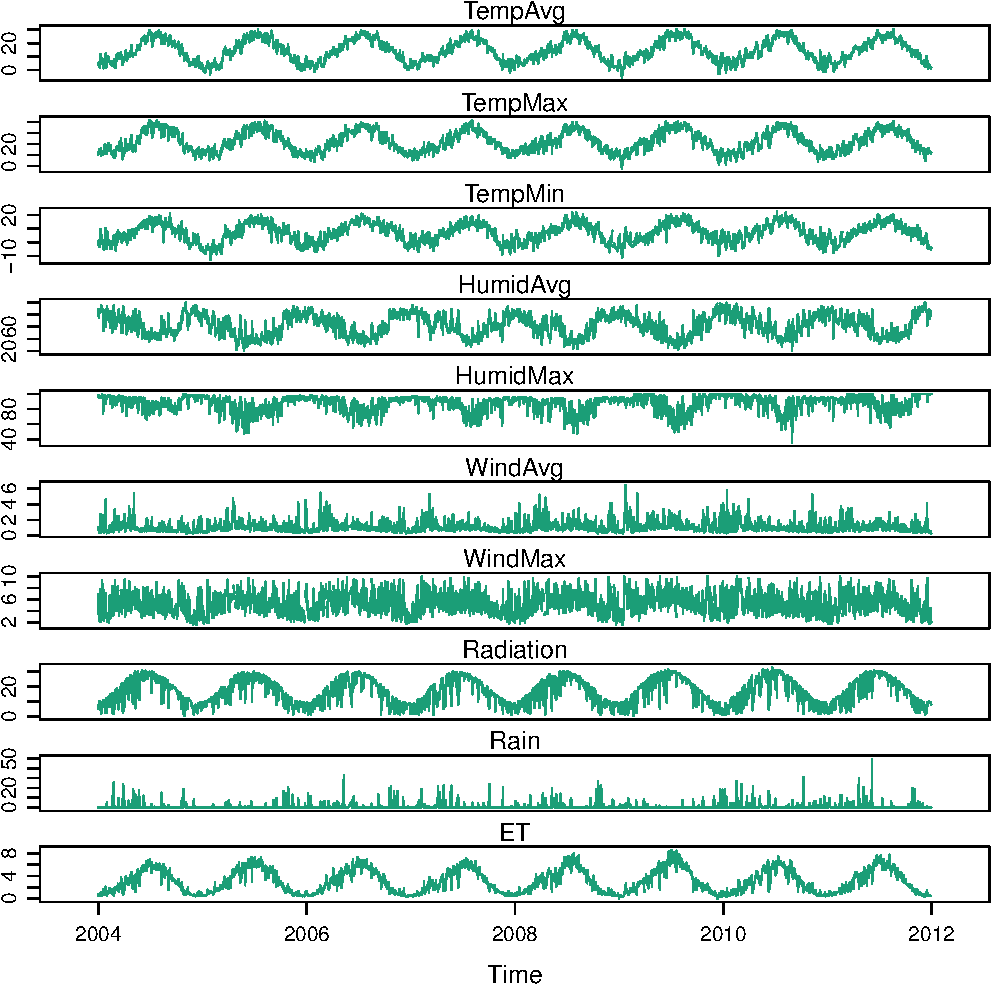
\includegraphics[width=.9\linewidth]{figs/aranjuez.pdf}
\caption{Time plot of the collection of meteorological time series of the Aranjuez station (\texttt{lattice} version). \label{fig:aranjuezNaive}}
\end{figure}

The package \texttt{ggplot2} provides the generic method \texttt{autoplot} to
automate the display of certain classes with a simple command. The
package \texttt{zoo} provides an \texttt{autoplot} method for the \texttt{zoo} class with a
result similar to that obtained with \texttt{xyplot} (Figure \ref{fig:aranjuezNaiveGG})

\lstset{language=r,label= ,caption= ,captionpos=b,numbers=none}
\begin{lstlisting}
  autoplot(aranjuez) + facet_free()
\end{lstlisting}

\begin{figure}[htbp]
\centering
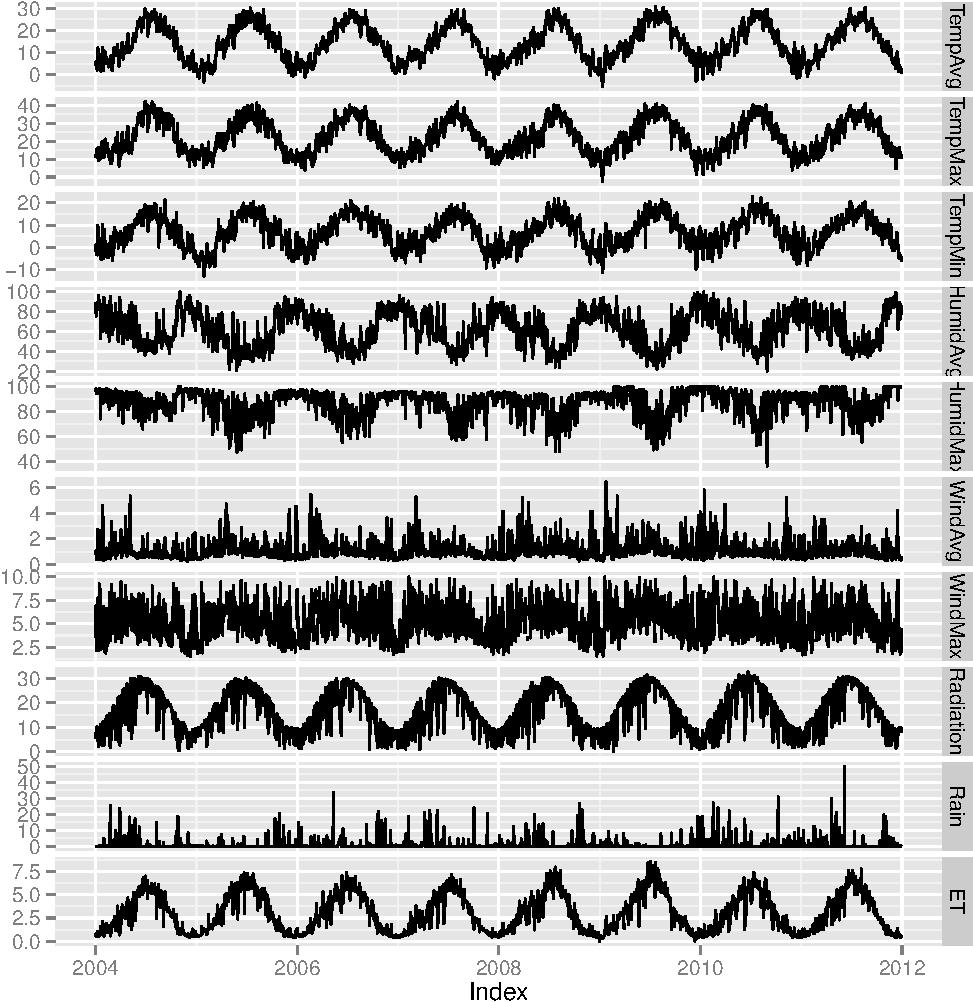
\includegraphics[width=.9\linewidth]{figs/aranjuezGG.pdf}
\caption{Time plot of the collection of meteorological time series of the Aranjuez station (\texttt{ggplot2} version). \label{fig:aranjuezNaiveGG}}
\end{figure}


\subsection{\floweroneleft Annotations to Enhance the Time Graph}
\label{sec:org07f591e}

These first attempts can be improved with a custom panel function
that generates the content of each panel using the information
processed by \texttt{xyplot}, or overlaying additional layers with
\texttt{autoplot}.  One of the main enhancements is to highlight certain time
regions that fulfill certain conditions. The package \texttt{latticeExtra}
provides a nice solution for \texttt{xyplot} with \texttt{panel.xblocks}. The result
is displayed in Figure \ref{fig:aranjuezEnhanced}:

\begin{itemize}
\item The label of each time series is displayed with text inside each
panel instead of using the strips mechanism. The \texttt{panel.text}
prints the name of each variable with the aid of \texttt{panel.number}.
\item The alternating of years is displayed with blocks of gray and
white color using the \texttt{panel.xblocks} function from
\texttt{latticeExtra}. The year is extracted (as character) from the
time index of the \texttt{zoo} object with \texttt{format.POSIXlt}.
\item Those values below the mean of each variable are highlighted
with short red color blocks at the bottom of each panel, again
with the \texttt{panel.xblocks} function.
\item The maxima and minima are highlighted with small blue triangles.
\end{itemize}

Because the functions included in the panel function are executed
consecutively, their order determines the superposition of graphical
layers.
\index{Panel function}
\index{panel.xblocks@\texttt{panel.xblocks}}
\index{panel.text@\texttt{panel.text}}
\index{panel.number@\texttt{panel.number}}
\index{panel.points@\texttt{panel.points}}

\lstset{language=r,label= ,caption= ,captionpos=b,numbers=none}
\begin{lstlisting}
  library(grid)
  library(latticeExtra)
  
  ## Auxiliary function to extract the year value of a POSIXct time
  ## index
  Year <- function(x)format(x, "%Y")
  
  xyplot(aranjuez, layout=c(1, ncol(aranjuez)), strip=FALSE,
         scales=list(y=list(cex=0.6, rot=0)),
         panel=function(x, y, ...){
           ## Alternation of years
           panel.xblocks(x, Year,
                         col = c("lightgray", "white"),
                         border = "darkgray")
           ## Values under the average highlighted with red regions
           panel.xblocks(x, y<mean(y, na.rm=TRUE),
                         col = "indianred1",
                         height=unit(0.1, 'npc'))
           ## Time series
           panel.lines(x, y, col='royalblue4', lwd=0.5, ...)
           ## Label of each time series
           panel.text(x[1], min(y, na.rm=TRUE),
                      names(aranjuez)[panel.number()],
                      cex=0.6, adj=c(0, 0), srt=90, ...)
           ## Triangles to point the maxima and minima 
           idxMax <- which.max(y)
           panel.points(x[idxMax], y[idxMax],
                        col='black', fill='lightblue', pch=24)
           idxMin <- which.min(y)
           panel.points(x[idxMin], y[idxMin],
                        col='black', fill='lightblue', pch=25)
         })
\end{lstlisting}

\begin{figure}[htbp]
\centering
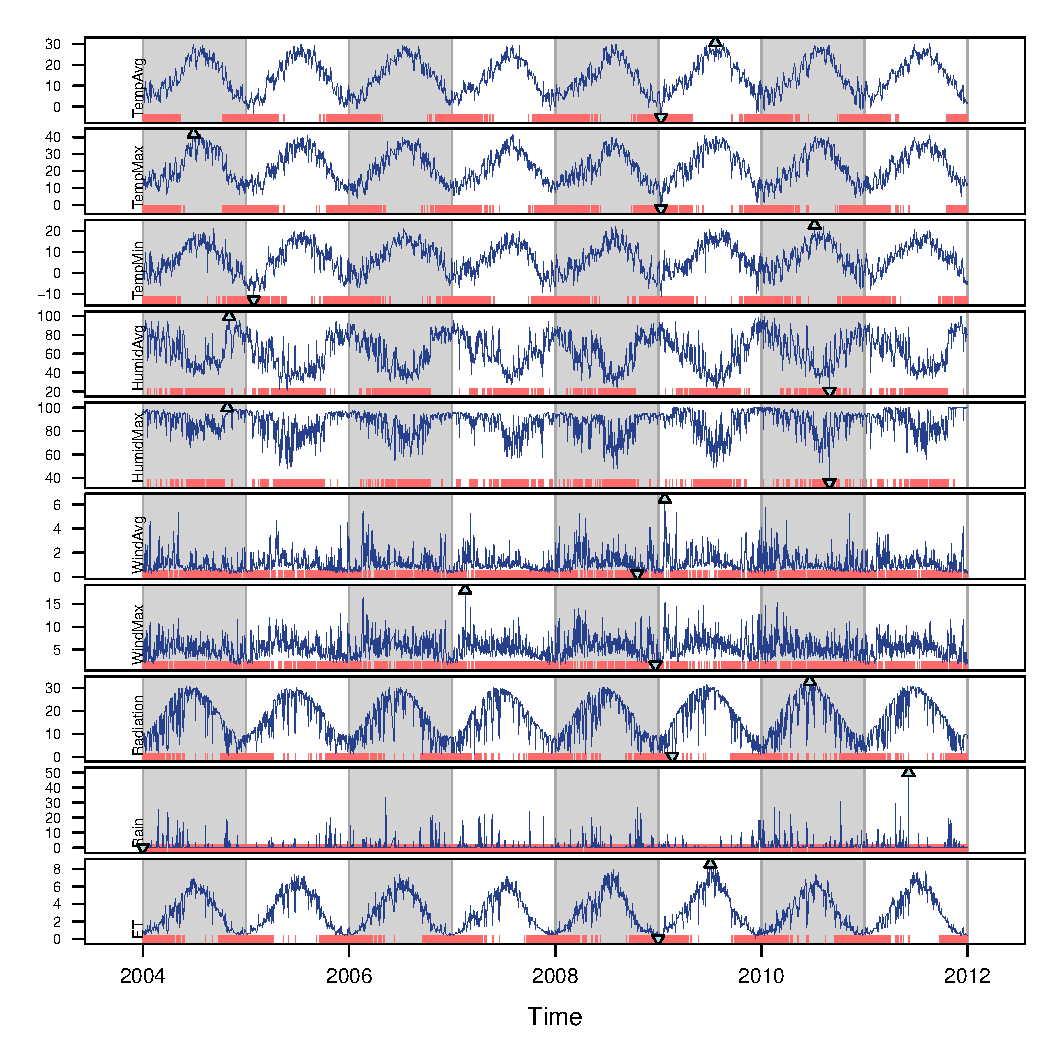
\includegraphics[width=.9\linewidth]{figs/aranjuezXblocks.pdf}
\caption{Enhanced time plot of the collection of meteorological time series of the Aranjuez station. \label{fig:aranjuezEnhanced}}
\end{figure}

There is no equivalent \texttt{panel.xblocks} function that can be used with
\texttt{ggplot2}. Therefore, the \texttt{ggplot2} version must explicitly compute
the corresponding bands (years and regions below the average values):

\begin{itemize}
\item The first step in working with \texttt{ggplot} is to transform the \texttt{zoo}
object into a \texttt{data.frame} in long format. \texttt{fortify} returns a
\texttt{data.frame} with three columns: the time \texttt{Index}, a factor
indicating the \texttt{Series}, and the corresponding \texttt{Value}.
\end{itemize}
\lstset{language=r,label= ,caption= ,captionpos=b,numbers=none}
\begin{lstlisting}
  timeIdx <- index(aranjuez)
  
  long <- fortify(aranjuez, melt=TRUE)
\end{lstlisting}

\begin{itemize}
\item The bands of values below the average can be easily extracted with
\texttt{scale} because these regions are negative when the \texttt{data.frame} is
centered.
\end{itemize}
\lstset{language=r,label= ,caption= ,captionpos=b,numbers=none}
\begin{lstlisting}
  ## Values below mean are negative after being centered
  scaled <- fortify(scale(aranjuez, scale=FALSE), melt=TRUE)
  ## The 'scaled' column is the result of the centering.
  ## The new 'Value' column store the original values.
  scaled <- transform(scaled, scaled=Value, Value=long$Value)
  underIdx <- which(scaled$scaled <= 0)
  ## 'under' is the subset of values below the average
  under <- scaled[underIdx,]
\end{lstlisting}

\begin{itemize}
\item The years bands are defined with the function \texttt{endpoints} from the
\texttt{xts} package:
\end{itemize}
\index{Package!xts@\texttt{xts}}
\lstset{language=r,label= ,caption= ,captionpos=b,numbers=none}
\begin{lstlisting}
  library(xts)
  ep <- endpoints(timeIdx, on='years')
  N <- length(ep[-1])
  ## 'tsp' is start and 'tep' is the end of each band
  tep <- timeIdx[ep]
  tsp <- timeIdx[ep[-(N+1)]+1]
  ## 'cols' is a vector with the color of each band
  cols <- rep_len(c('gray', 'white'), N)
\end{lstlisting}
\begin{itemize}
\item The minima and maxima points of each variable are extracted with
\texttt{apply}:
\end{itemize}
\lstset{language=r,label= ,caption= ,captionpos=b,numbers=none}
\begin{lstlisting}
  minIdx <- timeIdx[apply(aranjuez, 2, which.min)]
  minVals <- apply(aranjuez, 2, min, na.rm=TRUE)
  mins <- data.frame(Index=minIdx,
                     Value=minVals,
                     Series=names(aranjuez))
  
  maxIdx <- timeIdx[apply(aranjuez, 2, which.max)]
  maxVals <- apply(aranjuez, 2, max, na.rm=TRUE)
  maxs <- data.frame(Index=maxIdx,
                     Value=maxVals,
                     Series=names(aranjuez))
\end{lstlisting}

\begin{itemize}
\item With \texttt{ggplot} we define the canvas, and the layers of information are
added successively:
\end{itemize}
\lstset{language=r,label= ,caption= ,captionpos=b,numbers=none}
\begin{lstlisting}
  ggplot(data=long, aes(Index, Value)) +
      ## Time series of each variable
      geom_line(colour = "royalblue4", lwd = 0.5) +
      ## Year bands
      annotate(geom='rect', ymin = -Inf, ymax = Inf,
                xmin=tsp, xmax=tep,
                fill = cols, alpha = 0.4) +
      ## Values below average
      geom_rug(data=under,
               sides='b', col='indianred1') +
      ## Minima
      geom_point(data=mins, pch=25) +
      ## Maxima
      geom_point(data=maxs, pch=24) +
      ## Axis labels and theme definition
      labs(x='Time', y=NULL) +
      theme_bw() +
      ## Each series is displayed in a different panel with an
      ## independent y scale
      facet_free()
\end{lstlisting}

Some messages from Figure \ref{fig:aranjuezEnhanced}:
\begin{itemize}
\item The radiation, temperature, and evotranspiration are
quasi-periodic and are almost synchronized between them. Their
local maxima appear in the summer and the local minima in the
winter. Obviously, the summer values are higher than the
average.
\item The average humidity varies in oposition to the temperature and
radiation cycle, with local maxima located during winter.
\item The average and maximum wind speed, and rainfall vary in a more
erratic way and do not show the evident periodic behavior of
the radiation and temperature.
\item The rainfall is different from year to year. The remaining variables
do not show variations between years.
\item The fluctuations of solar radiation are more apparent than
the temperature fluctuations. There is hardly any day with
temperatures below the average value during summer, while it is
not difficult to find days with radiation below the average
during this season.
\end{itemize}

\section{Time Series of Variables with the Same Scale \label{SEC:sameScale}}
\label{sec:orgefc122a}
As an example of time series of variables with the same scale, we will
use measurements of solar radiation from different meteorological
stations.

The first attempt to display this multivariate time series makes use
of the \texttt{xyplot.zoo} method. The objective of this graphic is to
display the behavior of the collection as a whole: the series are
superposed in the same panel (\texttt{superpose=TRUE}) without legend
(\texttt{auto.key=TRUE}), using thin lines and partial
transparency\footnote{A similar result can be obtained with \texttt{autoplot} using \texttt{facets=NULL}.}. Transparency softens overplotting problems and reveals
density clusters because regions with more overlapping lines are
darker. Figure \ref{fig:navarraNaive} displays the variations
around the time average (\texttt{avRad}).

\lstset{language=r,label= ,caption= ,captionpos=b,numbers=none}
\begin{lstlisting}
  load('data/navarra.RData')
\end{lstlisting}


\index{zoo@\texttt{zoo}} 
\index{xyplot.zoo@\texttt{xyplot.zoo}}

\lstset{language=r,label= ,caption= ,captionpos=b,numbers=none}
\begin{lstlisting}
  avRad <- zoo(rowMeans(navarra, na.rm=1), index(navarra))
  pNavarra <- xyplot(navarra - avRad,
                     superpose=TRUE, auto.key=FALSE,
                     lwd=0.5, alpha=0.3, col='midnightblue') 
  pNavarra
\end{lstlisting}

\begin{figure}[htbp]
\centering
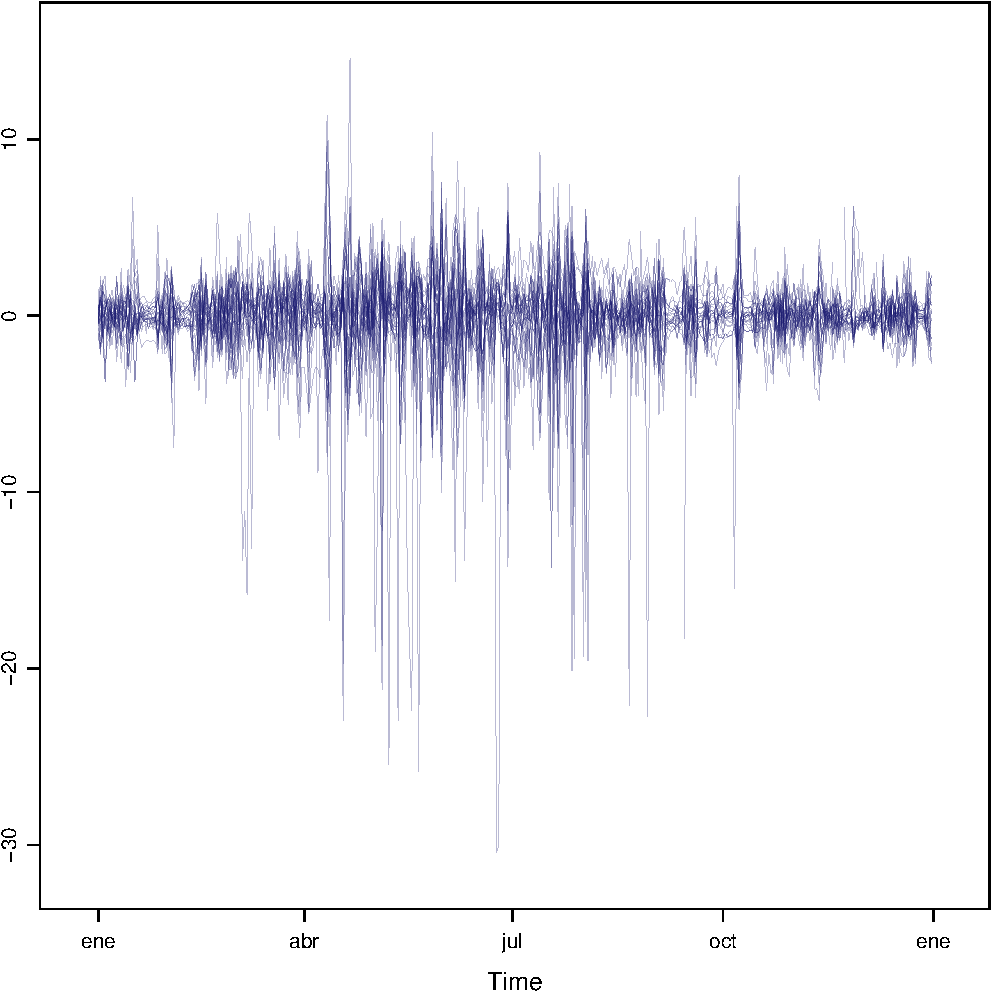
\includegraphics[width=.9\linewidth]{figs/navarra.pdf}
\caption{Time plot of the variations around time average of solar radiation measurements from the meteorological stations of Navarra. \label{fig:navarraNaive}}
\end{figure}

This result can be improved with different methods: the cut-and-stack
method, the horizon graph with \texttt{horizonplot}, and dynamic labeling
with the \texttt{gridSVG} package.

\subsection{Aspect Ratio and Rate of Change}
\label{sec:orgd2b8a0e}
When a graphic is intended to inform about the rate of change,
special attention must be paid to the aspect ratio of the graph,
defined as the ratio of the height to the width of the graphical
window. Cleveland analyzed the importance of the aspect ratio for
judging rate of change. He concluded that we visually decode the
information about the relative local rate of change of one
variable with another by comparing the orientations of the local
line segments that compose the polylines. The recommendation is to
choose the aspect ratio so that the absolute values of the
orientations of the segments are centered on \(\SI{45}{\degree}\) (banking
to \(\SI{45}{\degree}\)). 

The problem with banking to \(\SI{45}{\degree}\) is that the resulting
aspect ratio is frequently too small. A suitable solution to
minimize wasted space is the cut-and-stack method. The \texttt{xyplot.ts}
method implement this solution with the combination of the
arguments \texttt{aspect} and \texttt{cut}. The version of Figure
\ref{fig:navarraNaive} using banking to \(\SI{45}{\degree}\) and the
cut-and-stack method is produced with
\lstset{language=r,label= ,caption= ,captionpos=b,numbers=none}
\begin{lstlisting}
  xyplot(navarra - avRad,
         aspect='xy', cut=list(n=3, overlap=0.1),
         strip=FALSE,
         superpose=TRUE, auto.key=FALSE,
         lwd=0.5, alpha=0.3, col='midnightblue')
\end{lstlisting}

\begin{figure}[htbp]
\centering
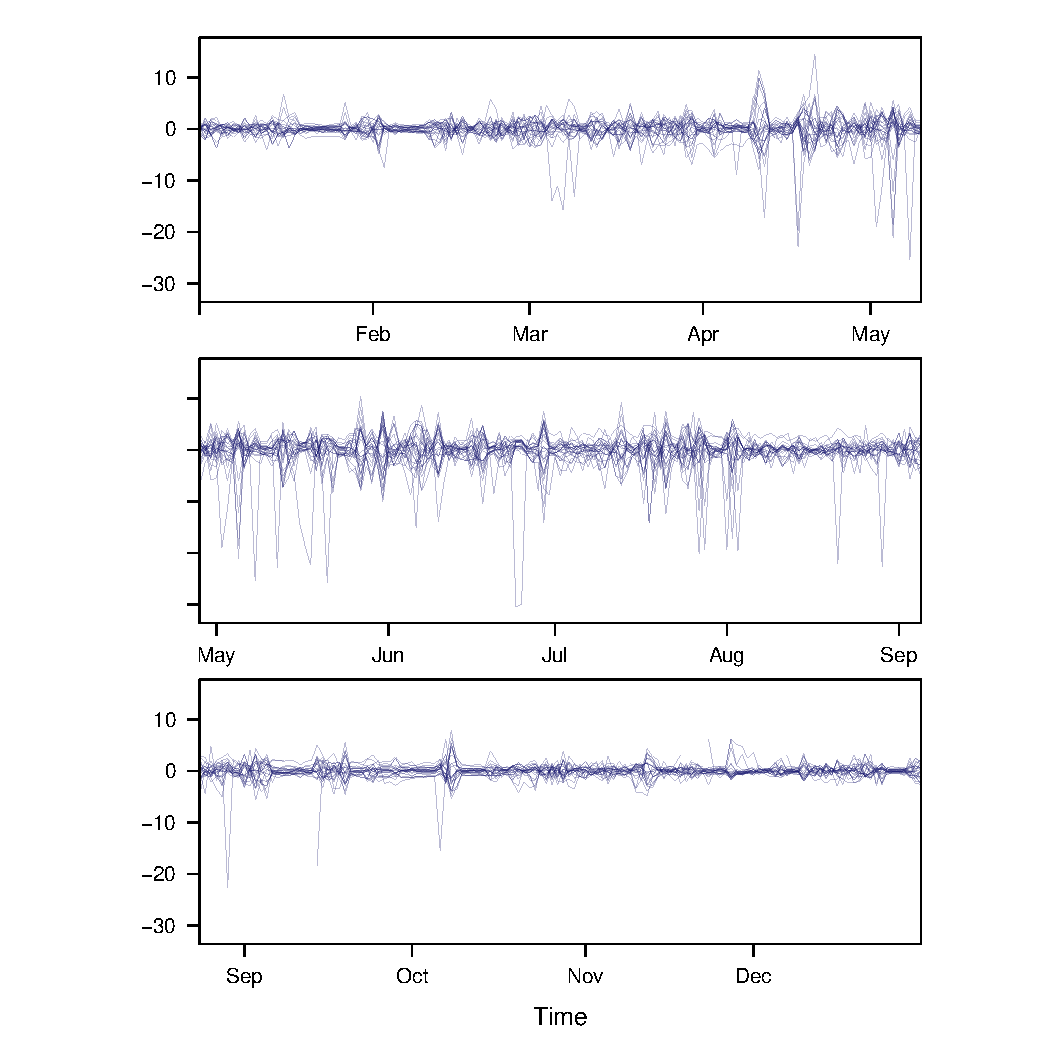
\includegraphics[width=.9\linewidth]{figs/navarraBanking.pdf}
\caption{Cut-and-stack plot with banking to \(\SI{45}{\degree}\). \label{fig:navarraBanking}}
\end{figure}

\subsection{The Horizon Graph \label{sec:horizonplot}}
\label{sec:orga0ff336}
The horizon graph\index{Horizon graph} is useful in examining how a
large number of series changes over time, and does so in a way
that allows both comparisons between the individual time series
and and independent analysis of each series. Moreover,
extraordinary behaviors and predominant patterns are easily
distinguished \cite{Heer.Kong.ea2009,Few2008}.

This graph displays several stacked series collapsing the y-axis
to free vertical space:
\begin{itemize}
\item Positive and negative values share the same vertical
space. Negative values are inverted and placed above the
reference line. Sign is encoded using different hues (positive
values in blue and negative values in red).
\item Differences in magnitude are displayed as differences in color
intensity (darker colors for greater differences).
\item The color bands share the same baseline and are superposed, with
darker bands in front of the ligther ones.
\end{itemize}

Because the panels share the same design structure, once this
technique is understood, it is easy to establish comparisons or spot
extraordinary events.  This method is what Tufte described as small
multiples\index{Small multiples} \cite{Tufte1990}.

Figure \ref{fig:navarraHorizonplot} displays the variations of
solar radiation around the time average with an horizon graph
using a row for each time series.

\index{Packages!latticeExtra@\texttt{latticeExtra}}
\index{horizonplot@\texttt{horizonplot}}

\lstset{language=r,label= ,caption= ,captionpos=b,numbers=none}
\begin{lstlisting}
  library(latticeExtra)
  
  horizonplot(navarra-avRad,
              layout=c(1, ncol(navarra)),
              origin=0, colorkey=TRUE)
\end{lstlisting}

\begin{figure}[htbp]
\centering
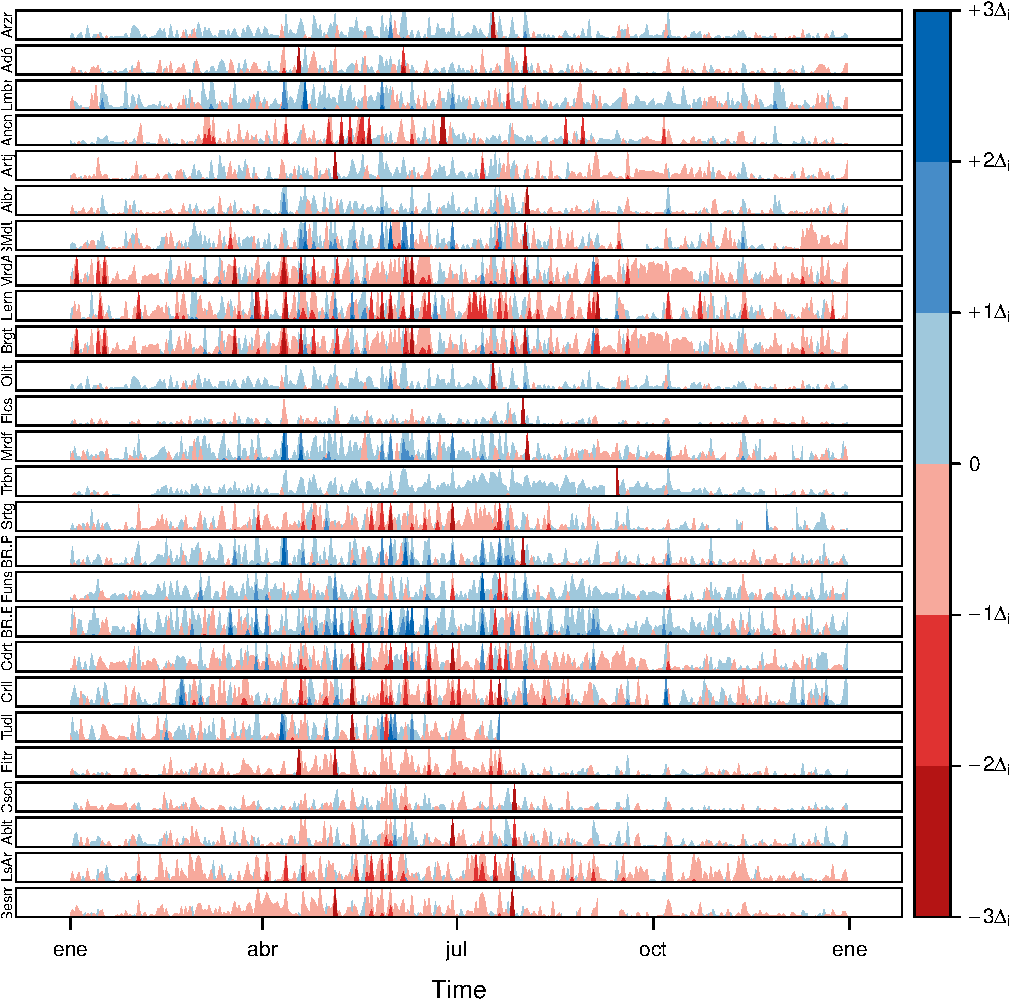
\includegraphics[width=.9\linewidth]{figs/navarraHorizonplot.pdf}
\caption{Horizon plot of variations around time average of solar radiation measurements from the meteorological stations of Navarra. \label{fig:navarraHorizonplot}}
\end{figure}

Figure \ref{fig:navarraHorizonplot} allows several questions to be
answered:
\begin{itemize}
\item Which stations consistently measure above and below the average?
\item Which stations resemble more closely the average time series?
\item Which stations show erratic and uniform behavior?
\item In each of the stations, is there any day with extraordinary measurements?
\item Which part of the year is associated with more intense
absolute fluctuations across the set of stations?
\end{itemize}

\subsection{Time Graph of the Differences between a Time Series and a Reference \label{sec:differences}}
\label{sec:org7d979d9}

The horizon graph is also useful in revealing the differences between
a univariate time series and another reference. For example, we
might be interested in the departure of the observed temperature
from the long-term average, or in other words, the temperature
change over time.

Let's illustrate this approach with the time series of daily
average temperatures measured at the meteorological station of
Aranjuez. The reference is the long-term daily average calculated
with \texttt{ave}.

\lstset{language=r,label= ,caption= ,captionpos=b,numbers=none}
\begin{lstlisting}
  Ta <- aranjuez$TempAvg
  timeIndex <- index(aranjuez)
  longTa <- ave(Ta, format(timeIndex, '%j'))
  diffTa <- (Ta - longTa)
\end{lstlisting}


The temperature time series, the long-term average and the
differences between them can be displayed with the \texttt{xyplot}
method, now using \texttt{screens} to use a different panel for the
differences time series (Figure \ref{fig:diffTa_xyplot})
\lstset{language=r,label= ,caption= ,captionpos=b,numbers=none}
\begin{lstlisting}
  xyplot(cbind(Ta, longTa, diffTa),
         col=c('darkgray', 'red', 'midnightblue'),
         superpose=TRUE, auto.key=list(space='right'),
         screens=c(rep('Average Temperature', 2), 'Differences'))
\end{lstlisting}

\begin{figure}[htbp]
\centering
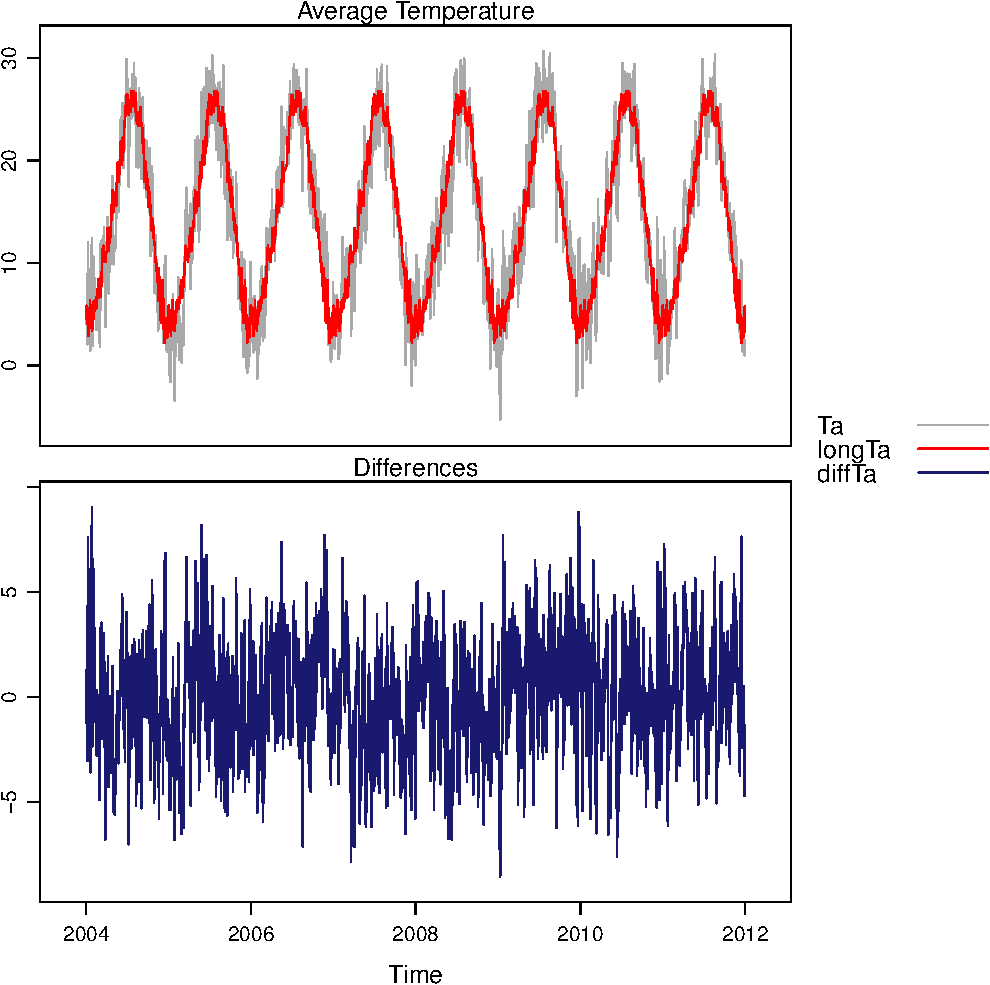
\includegraphics[width=.9\linewidth]{figs/diffTa_xyplot.pdf}
\caption{Daily temperature time series, its long-term average and the differences between them. \label{fig:diffTa_xyplot}}
\end{figure}

The horizon graph is better suited for displaying the differences. The
next code again uses the cut-and-stack method (Figure
\ref{fig:navarraBanking}) to distinguish between years. Figure
\ref{fig:diffTa_horizon} shows that 2004 started clearly above the
average while 2005 and 2009 did the contrary. Year 2007 was frequently
below the long-term average but 2011 was more similar to that
reference.
\lstset{language=r,label= ,caption= ,captionpos=b,numbers=none}
\begin{lstlisting}
  years <- unique(format(timeIndex, '%Y'))
  
  horizonplot(diffTa, cut=list(n=8, overlap=0),
              colorkey=TRUE, layout=c(1, 8),
              scales=list(draw=FALSE, y=list(relation='same')),
              origin=0, strip.left=FALSE) +
      layer(grid.text(years[panel.number()], x = 0, y = 0.1, 
                      gp=gpar(cex=0.8),
                      just = "left"))
\end{lstlisting}

\begin{figure}[htbp]
\centering
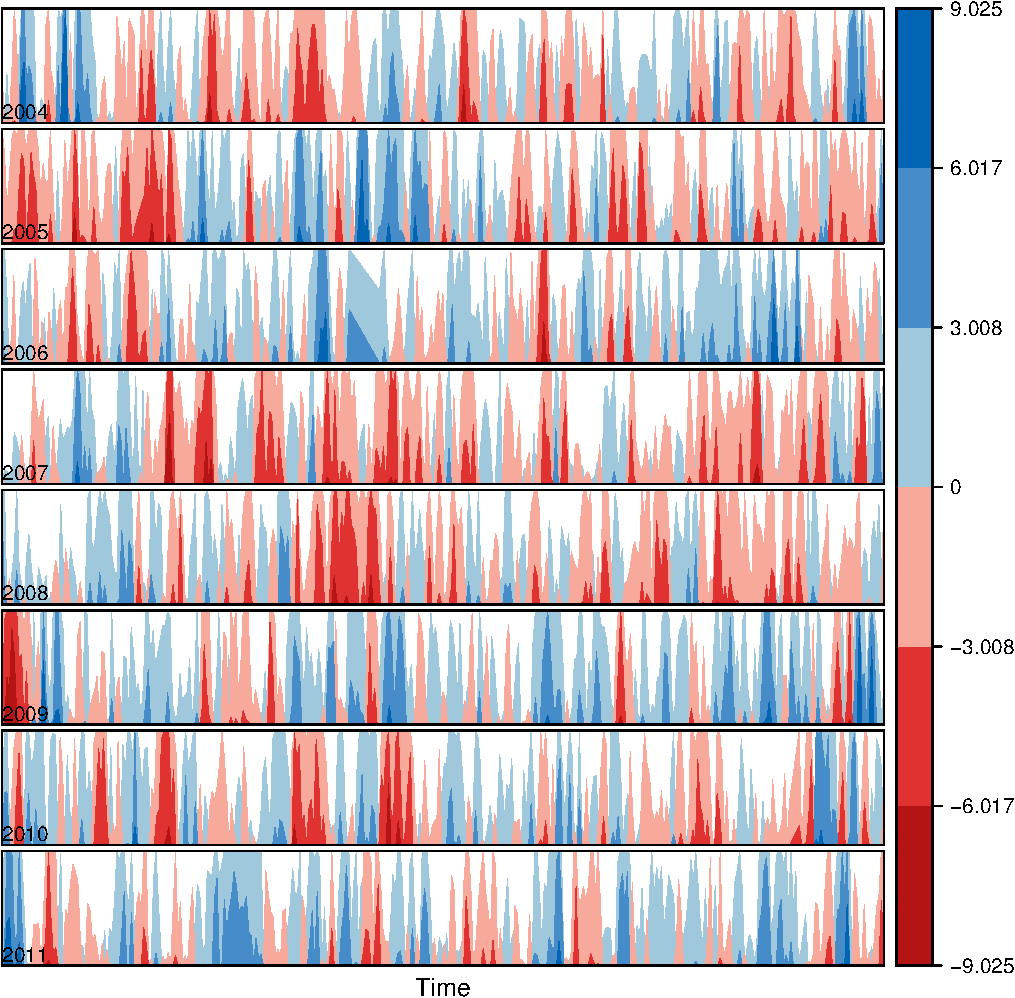
\includegraphics[width=.9\linewidth]{figs/diffTa_horizon.pdf}
\caption{Horizon graph displaying differences between a daily temperature time series and its long-term average. \label{fig:diffTa_horizon}}
\end{figure}

A different approach to display this information is to produce a level
plot displaying the time series using parts of its time index as
independent and conditioning variables\footnote{This approach was inspired by the \texttt{strip} function of the
\texttt{metvurst} package
\url{https://metvurst.wordpress.com/2013/03/04/visualising-large-amounts-of-hourly-environmental-data-2/}.}. The following code
displays the differences with the day of month on the horizontal axis
and the year on the vertical axis, with a different panel for each
month number. Therefore, each cell of Figure \ref{fig:diffTa_level}
corresponds to a certain day of the time series. If you compare this
figure with the horizon plot, you will find the same previous findings
but revealed now in more detail. On the other hand, while the horizon
plot of Figure \ref{fig:diffTa_horizon} clearly displays the yearly
evolution, the combination of variables of the level plot focuses on
the comparison between years in a certain month.

\lstset{language=r,label= ,caption= ,captionpos=b,numbers=none}
\begin{lstlisting}
  year <- function(x)as.numeric(format(x, '%Y'))
  day <- function(x)as.numeric(format(x, '%d'))
  month <- function(x)as.numeric(format(x, '%m'))
\end{lstlisting}

\lstset{language=r,label= ,caption= ,captionpos=b,numbers=none}
\begin{lstlisting}
  myTheme <- modifyList(custom.theme(region=brewer.pal(9, 'RdBu')),
                                     list(
                                       strip.background=list(col='gray'),
                                       panel.background=list(col='gray')))
  
  maxZ <- max(abs(diffTa))
  
  levelplot(diffTa ~ day(timeIndex) * year(timeIndex) | factor(month(timeIndex)),
            at=pretty(c(-maxZ, maxZ), n=8),
            colorkey=list(height=0.3),
            layout=c(1, 12), strip=FALSE, strip.left=TRUE,
            xlab='Day', ylab='Month', 
            par.settings=myTheme)
  
\end{lstlisting}

\begin{figure}[htbp]
\centering
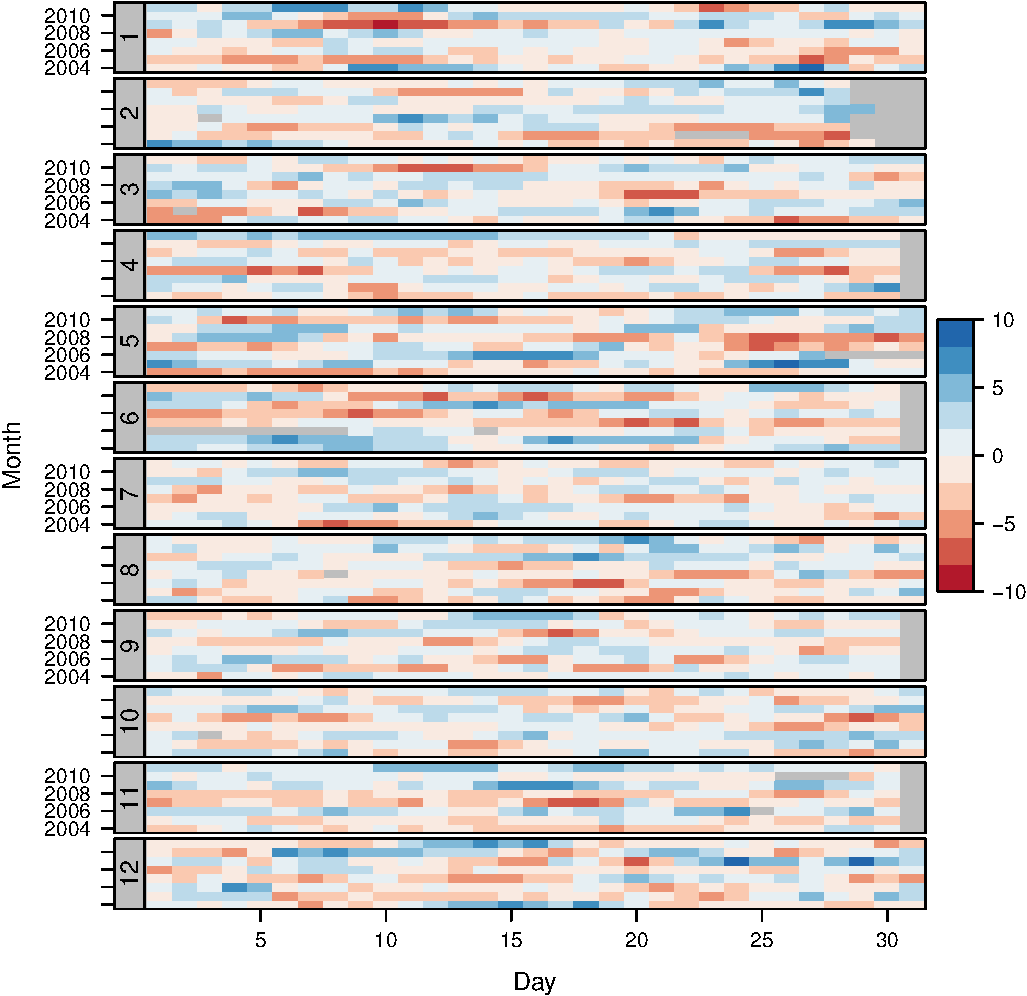
\includegraphics[width=.9\linewidth]{figs/diffTa_levelplot.pdf}
\caption{Level plot of differences between a daily temperature time series and its long-term average. \label{fig:diffTa_level}}
\end{figure}

ggplot version.
\lstset{language=r,label= ,caption= ,captionpos=b,numbers=none}
\begin{lstlisting}
df <- data.frame(Vals = diffTa,
                 Day = day(timeIndex),
                 Year = year(timeIndex),
                 Month = month(timeIndex))

ggplot(data = df,
       aes(fill = Vals,
           x = Day,
           y = Year)) +
    facet_wrap(~ Month, ncol = 1, switch = 'y') +
    scale_y_continuous(breaks = pretty_breaks()) + 
    scale_fill_distiller(palette = 'RdBu', direction = 1) + 
    geom_tile(color = "white", size = 0.4) +
    theme(panel.grid.major = element_blank(),
          panel.grid.minor = element_blank())
\end{lstlisting}


\section{Interactive}
\label{sec:orgbc06b9a}

\subsection{Dygraphs \label{sec:dygraphs}}
\label{sec:orgaf87588}
\lstset{language=r,label= ,caption= ,captionpos=b,numbers=none}
\begin{lstlisting}
library(dygraphs)

dyTemp <- dygraph(aranjuez[, c("TempMin", "TempAvg", "TempMax")],
                  main = "Temperature in Aranjuez",
                  ylab = "ºC")

dyTemp
\end{lstlisting}

\lstset{language=r,label= ,caption= ,captionpos=b,numbers=none}
\begin{lstlisting}
dyTemp %>%
    dyHighlight(highlightSeriesBackgroundAlpha = 0.2)
\end{lstlisting}

\lstset{language=r,label= ,caption= ,captionpos=b,numbers=none}
\begin{lstlisting}
dyTemp %>%
    dyHighlight(highlightSeriesOpts = list(strokeWidth = 2))
\end{lstlisting}

\lstset{language=r,label= ,caption= ,captionpos=b,numbers=none}
\begin{lstlisting}
dygraph(aranjuez[, c("TempMin", "TempAvg", "TempMax")],
        main = "Temperature in Aranjuez",
        ylab = "ºC") %>%
    dySeries(c("TempMin", "TempAvg", "TempMax"),
             label = "Temperature")
\end{lstlisting}

\subsection{Highcharter \label{sec:highcharter}}
\label{sec:orgcb3d21e}

\lstset{language=r,label= ,caption= ,captionpos=b,numbers=none}
\begin{lstlisting}
library(highcharter)
library(xts)

aranjuezXTS <- as.xts(aranjuez)

highchart() %>%
    hc_add_series_xts(name = 'TempMax',
                      aranjuezXTS[, "TempMax"]) %>%
    hc_add_series_xts(name = 'TempMin',
                      aranjuezXTS[, "TempMin"]) %>%
    hc_add_series_xts(name = 'TempAvg',
                      aranjuezXTS[, "TempAvg"])

\end{lstlisting}

\subsection{plotly \label{sec:plotly}}
\label{sec:orgf41c7ac}

\lstset{language=r,label= ,caption= ,captionpos=b,numbers=none}
\begin{lstlisting}
library(reshape2)
df <- fortify(navarra - avRad)
df <- melt(df, id.vars = 'Index', variable.name = 'Station')
\end{lstlisting}

\lstset{language=r,label= ,caption= ,captionpos=b,numbers=none}
\begin{lstlisting}
## Number of stations
N <- ncol(navarra)
## Color palette
pal <- colorRampPalette(
    brewer.pal(9, 'Set1'))(N)
\end{lstlisting}

\lstset{language=r,label= ,caption= ,captionpos=b,numbers=none}
\begin{lstlisting}
library(plotly)

plot_ly(df,
        x = ~ Index,
        y = ~ value,
        color = ~ Station) %>%
    add_lines(alpha = 0.5, colors = pal)
\end{lstlisting}

\subsection{\floweroneleft Interaction with \texttt{gridSVG}}
\label{sec:org448ed5d}
The \texttt{gridSVG} package provides functions to convert \texttt{grid}-based \texttt{R}
graphics to an SVG format. It provides several functions to add
dynamic and interactive capabilities to \texttt{R} graphics. In this section
we will use \texttt{grid.script}, a function to add JavaScript code to a
plot.

The first step is to specify which component of the scene
will run the JavaScript code. The \texttt{grid.ls} function  returns a
listing of the names of grobs or viewports included in the graphic
output: only the lines will be connected with the JavaScript
code. 

\index{Packages!gridSVG@\texttt{gridSVG}}
\index{grid.ls@\texttt{grid.ls}}

\lstset{language=r,label= ,caption= ,captionpos=b,numbers=none}
\begin{lstlisting}
  library(gridSVG)
  ## grobs in the graphical output
  pNavarra
  grobs <- grid.ls(print=FALSE)
  ## only interested in some of them
  nms <- grobs$name[grobs$type == "grobListing"]
  idxNames <- grep('lines', nms)
  IDs <- nms[idxNames]
\end{lstlisting}

The second step is to modify each \texttt{grob} (graphical object) to add
attributes that specify when it will call JavaScript code. For each
line identified with the elements of the \texttt{IDs} vector and associated
to a meteorological station, the \texttt{navarra} object is accessed to
extract the annual mean value of the daily radiation and the
abbreviated name of the corresponding station (\texttt{info}).  The
\texttt{grid.garnish} function adds attributes to the \texttt{grob} of each line so
that when the mouse moves over a \texttt{grob}, the line is highlighted and
colored in red (\texttt{highlight}). When the mouse hovers out of the \texttt{grob},
the \texttt{hide} function sets back the default values of line width and
transparency, but uses the green color to denote that this line has
been already visited. In addition, because the browsers display the
content of the title attribute with a default tooltip, \texttt{grid.garnish}
sets this attribute to \texttt{info}.

\index{grid.garnish@\texttt{grid.garnish}}

\lstset{language=r,label= ,caption= ,captionpos=b,numbers=none}
\begin{lstlisting}
  for (id in unique(IDs)){
    ## extract information from the data
    ## according to the ID value
    i <- strsplit(id, '\\.')
    i <- sapply(i, function(x)as.numeric(x[5]))
    ## Information to be attached to each line: annual mean of daily
    ## radiation and abbreviated name of the station
    dat <- round(mean(navarra[,i], na.rm=TRUE), 2)
    info <- paste(names(navarra)[i], paste(dat, collapse=','),
                  sep=': ')
    ## attach SVG attributes
    grid.garnish(id,
                 onmouseover="highlight(evt)",
                 onmouseout="hide(evt)",
                 title=info)
  }
\end{lstlisting}

These JavaScript functions are included in a script file named
\texttt{highlight.js} (available at the website of the book). It can be
added as an additional object with \texttt{grid.script}.

\index{grid.script@\texttt{grid.script}}

\lstset{language=r,label= ,caption= ,captionpos=b,numbers=none}
\begin{lstlisting}
  grid.script(filename="highlight.js")
\end{lstlisting}

This script is easy to understand, even without previous
JavaScript knowledge:
\index{JavaScript}
\begin{verbatim}
  highlight = function(evt){',
      evt.target.setAttribute('opacity', '1');
      evt.target.setAttribute('stroke', 'red');
      evt.target.setAttribute('stroke-width', '1');
  }
  
  hide = function(evt){
      evt.target.setAttribute('opacity', '0.3');
      evt.target.setAttribute('stroke', green');
      evt.target.setAttribute('stroke-width', '0.3');
  }
\end{verbatim}

Finally, \texttt{gridToSVG} exports the whole scene to SVG. 
\index{grid.export@\texttt{grid.export}} 

\lstset{language=r,label= ,caption= ,captionpos=b,numbers=none}
\begin{lstlisting}
  grid.export('figs/navarraRadiation.svg')
\end{lstlisting}

A snapshot of the result, as viewed in a browser with a line
highlighted, is shown in Figure \ref{fig:navarraSVG}. Open the SVG
file with your browser, explore it using the horizon graph (Figure
\ref{fig:navarraHorizonplot}) as a reference, and try to answer the
questions raised with that graphic.

\begin{figure}
  \centering
  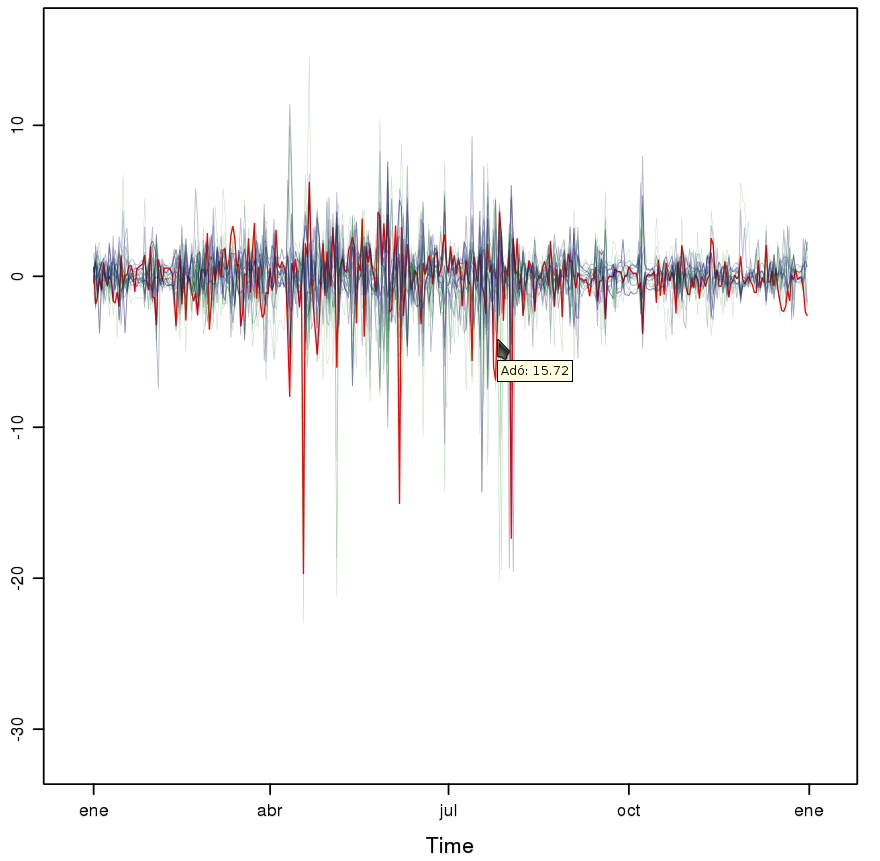
\includegraphics[width=0.9\textwidth]{figs/navarraSVG_captura.png}
  \caption{\label{fig:navarraSVG}Snapshot of an SVG graphic produced with \texttt{gridSVG}.}
\end{figure}



\section{Stacked Graphs \label{sec:stacked}}
\label{sec:org9fc194d}
If the variables of a multivariate time series can be summed to
produce a meaningful global variable, they may be better displayed
with stacked graphs. For example, the information on unemployment in
the United States provides data of unemployed persons by industry and
class of workers, and can be summed to give a total unemployment time
series.

\lstset{language=r,label= ,caption= ,captionpos=b,numbers=none}
\begin{lstlisting}
  load('data/unemployUSA.RData')
\end{lstlisting}

The time series of unemployment can be directly displayed
with the \texttt{xyplot.zoo} method (Figure \ref{fig:unemployUSAxyplot}).

\lstset{language=r,label= ,caption= ,captionpos=b,numbers=none}
\begin{lstlisting}
  xyplot(unemployUSA, superpose=TRUE, par.settings=custom.theme,
         auto.key=list(space='right'))
\end{lstlisting}

\begin{figure}[htbp]
\centering
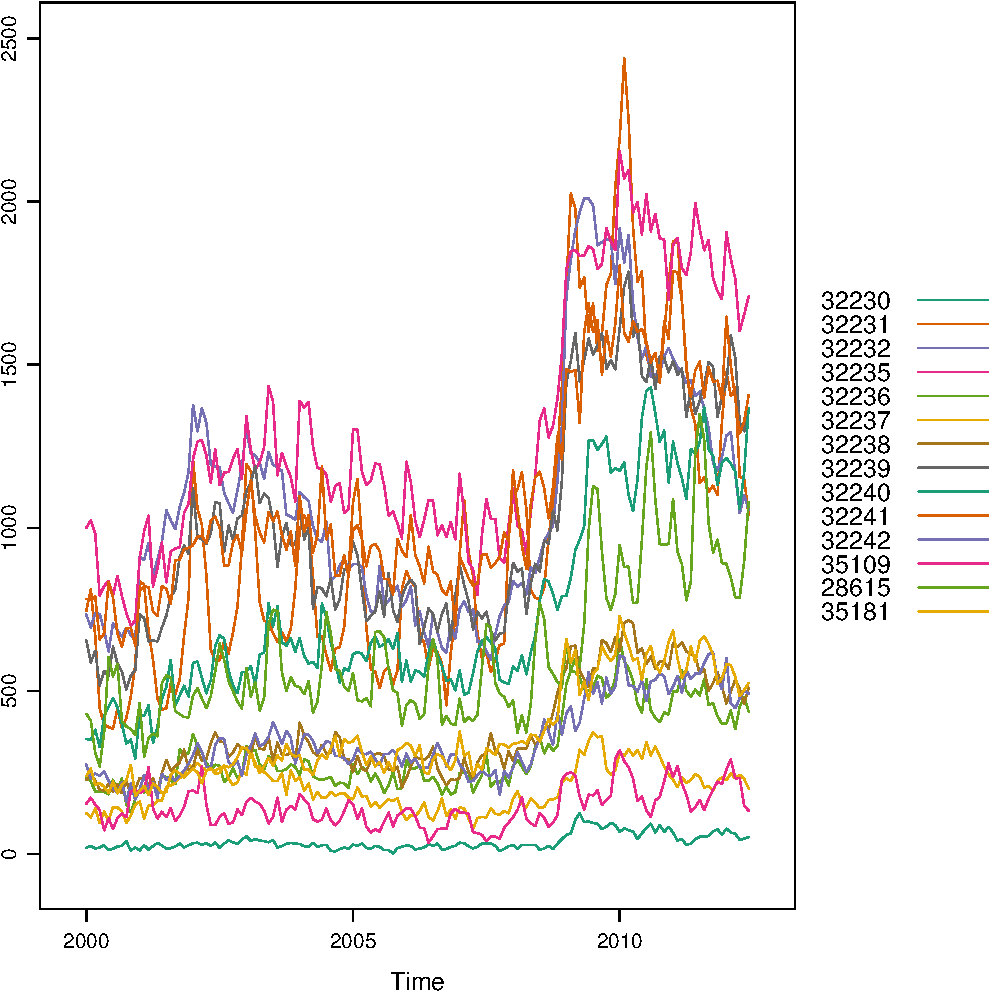
\includegraphics[width=.9\linewidth]{figs/unemployUSAxyplot.pdf}
\caption{Time series of unemployment  with \texttt{xyplot} using the default panel function. \label{fig:unemployUSAxyplot}}
\end{figure}

This graphical output is not very useful: the legend is confusing,
with too many items; the vertical scale is dominated by the largest
series, with several series buried in the lower part of the scale; the
trend, variations and structure of the total and individual
contributions cannot be deduced from this graph.

A suitable improvement is to display the multivariate time series as a
set of stacked colored polygons to follow the macro/micro principle
proposed by Tufte \cite{Tufte1990}: Show a collection of individual
time series and also display their sum. A traditional stacked graph is
easily obtained with \texttt{geom\_area} (Figure \ref{fig:unemployUSAgeomArea}):

\lstset{language=r,label= ,caption= ,captionpos=b,numbers=none}
\begin{lstlisting}
  library(scales) ## scale_x_yearmon needs scales::pretty_breaks
  autoplot(unemployUSA, facets=NULL, geom='area') +
      geom_area(aes(fill=Series)) +
      scale_x_yearmon()  
\end{lstlisting}

\begin{figure}[htbp]
\centering
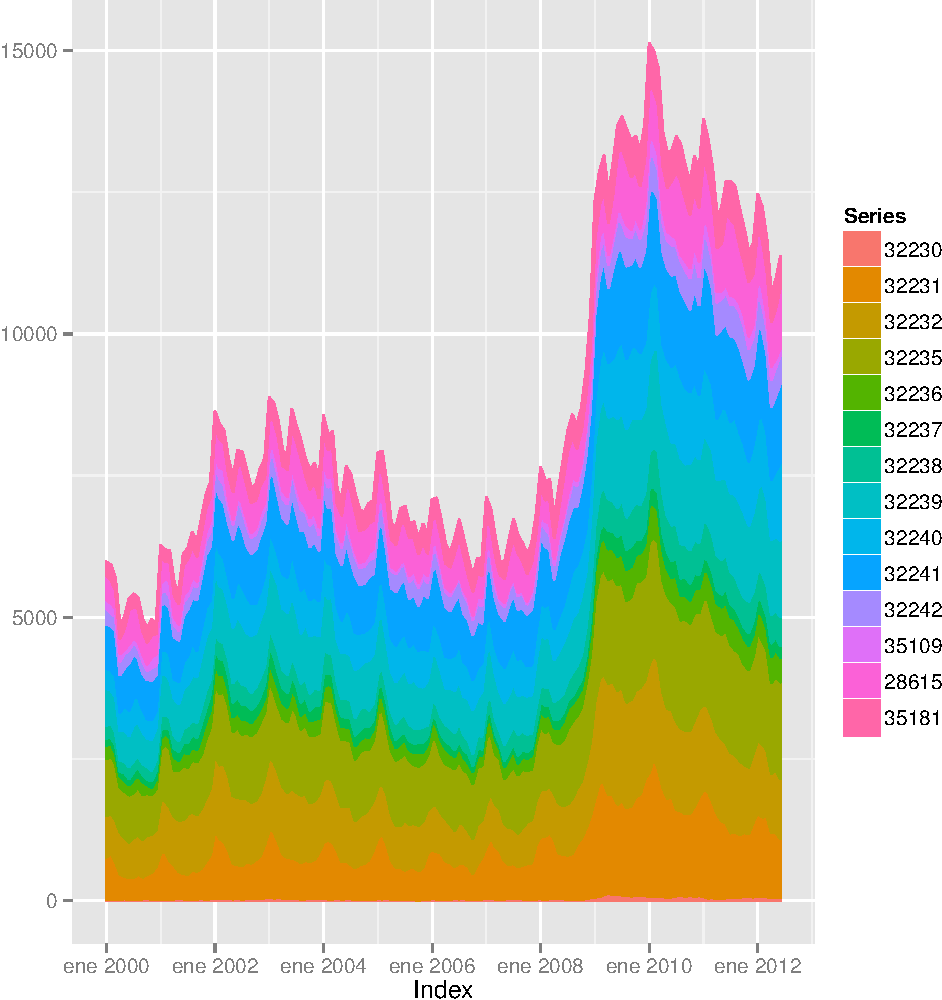
\includegraphics[width=.9\linewidth]{figs/unemployUSAgeomArea.pdf}
\caption{Time series of unemployment with stacked areas using \texttt{geom\_area}. \label{fig:unemployUSAgeomArea}}
\end{figure}

Traditional stacked graphs have their bottom on the x-axis which makes
the overall height at each point easy to estimate. On the other hand,
with this layout, individual layers may be difficult to
distinguish. The \emph{ThemeRiver} \cite{Havre.Hetzler.ea2002} (also named
\emph{streamgraph} in \cite{Byron.Wattenberg2008}) provides an innovative
layout method in which layers are symmetrical around the x-axis at
their center. At a glance, the pattern of the global sum and
individual variables, their contribution to conform the global sum,
and the interrelation between variables can be perceived.

I have defined a panel and prepanel functions\footnote{The code of these panel and prepanel functions is explained
in Section \ref{sec:themeRiverPanel}.} to implement a
ThemeRiver with \texttt{xyplot}. The result is displayed in Figure
\ref{fig:unemployUSAThemeRiver} with a vertical line to indicate
one of main milestones of the financial crisis, whose effect on
the overall unemployment results is clearly evident.
\lstset{language=r,label= ,caption= ,captionpos=b,numbers=none}
\begin{lstlisting}
  library(colorspace)
  ## We will use a qualitative palette from colorspace
  nCols <- ncol(unemployUSA)
  pal <- rainbow_hcl(nCols, c=70, l=75, start=30, end=300)
  myTheme <- custom.theme(fill=pal, lwd=0.2)
  
  sep2008 <- as.numeric(as.yearmon('2008-09'))
  
  xyplot(unemployUSA, superpose=TRUE, auto.key=FALSE,
         panel=panel.flow, prepanel=prepanel.flow,
         origin='themeRiver', scales=list(y=list(draw=FALSE)),
         par.settings=myTheme) +
      layer(panel.abline(v=sep2008, col='gray', lwd=0.7))
\end{lstlisting}

\begin{figure}[htbp]
\centering
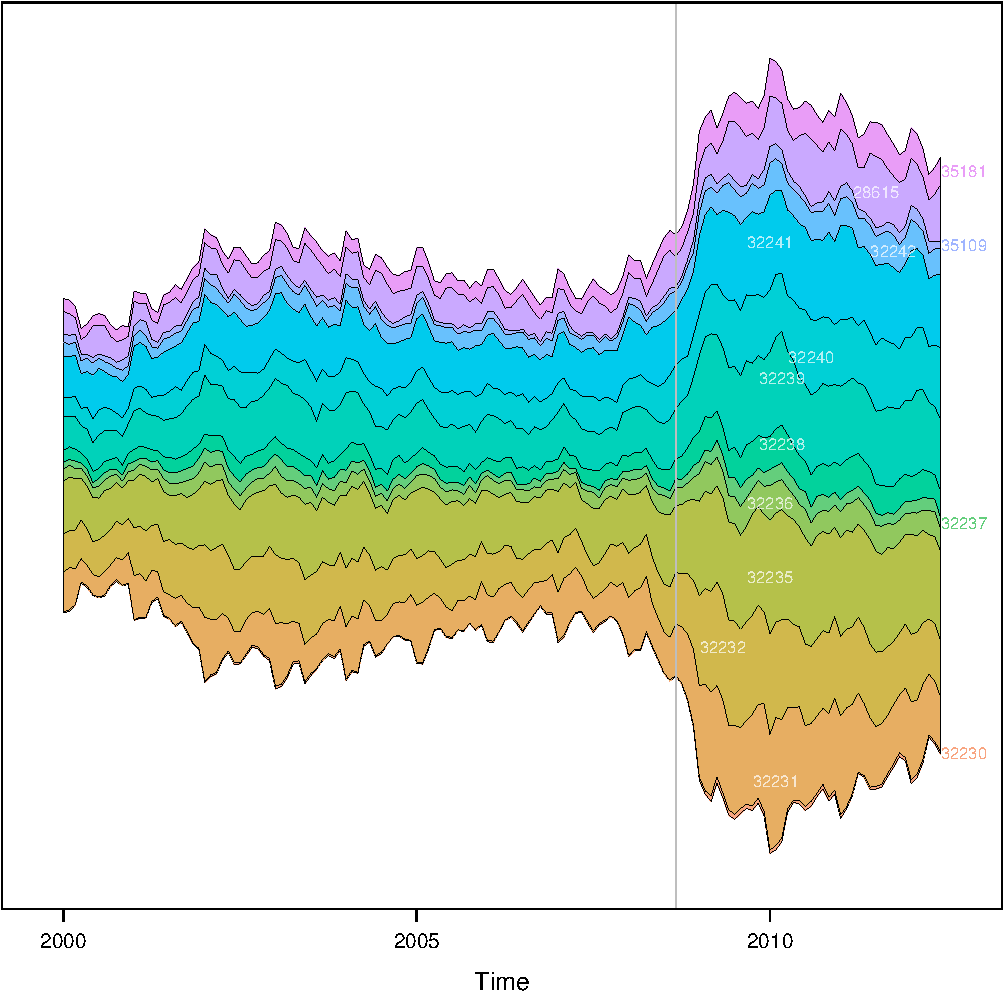
\includegraphics[width=.9\linewidth]{figs/unemployUSAThemeRiver.pdf}
\caption{ThemeRiver of unemployment in the United States. \label{fig:unemployUSAThemeRiver}}
\end{figure}

This figure can help answer several questions. For example:
\begin{itemize}
\item What is the industry or class of worker with the lowest/highest
unemployment figures during this time period?
\item What is the industry or class of worker with the lowest/highest
unemployment increases due to the financial crisis?
\item There are a number of local maxima and minima of the total
unemployment numbers. Are all the classes contributing to the
maxima/minima?  Do all the classes exhibit the same fluctuation
behavior as the global evolution?
\end{itemize}
More questions and answers can be found in the ``Current Employment
Statistics'' reports from the Bureau of Labor Statistics\footnote{The March 2012 highlights report is available at \url{http://www.bls.gov/ces/highlights032012.pdf}.}.



\subsection{\floweroneleft Panel and Prepanel Functions to Implement the ThemeRiver with \texttt{xyplot} \label{sec:themeRiverPanel}}
\label{sec:org327f4fe}
The \texttt{xyplot} function displays information according to the class
of its first argument (methods) and to the \texttt{panel} function. We
will use the \texttt{xyplot.zoo} method (equivalent to the \texttt{xyplot.ts}
method) with a new custom \texttt{panel} function.  This new panel
function has four main arguments, three of them calculated by
\texttt{xyplot} (\texttt{x}, \texttt{y} and \texttt{groups}) and a new one, \texttt{origin}. Of
course, it includes the \texttt{...} argument to provide additional
arguments.

The first step is to create a \texttt{data.frame} with coordinates and with
the \texttt{groups} factor. The value and number of the levels will be used
in the main step of this \texttt{panel} function. With this \texttt{data.frame} we
have to calculate the \texttt{y} and \texttt{x} coordinates for each group to get a
stacked set of polygons.

This \texttt{data.frame} is in the \emph{long} format, with a row for each
observation, and where the \texttt{group} column identifies the
variable. Thus, it must be transformed to the \emph{wide} format, with a
column for each variable. With the \texttt{unstack} function, a new
\texttt{data.frame} is produced whose columns are defined according to the
formula \texttt{y \textasciitilde{} groups} and with a row for each time position. The stack
of polygons is the result of the cumulative sum of each row
(\texttt{apply(yWide, 1, cumsum)}). The origin of this sum is defined with
the corresponding \texttt{origin} argument: with \texttt{themeRiver}, the polygons
are arranged in a symmetric way.

Each column of this matrix of cumulative sums defines the \texttt{y}
coordinate of each variable (where \texttt{origin} is now the first
variable). The polygon of each variable is between this curve
(\texttt{iCol+1}) and the one of the previous variable (\texttt{iCol}). In order to
get a closed polygon, the coordinates of the inferior limit are in
reverse order. This new \texttt{data.frame} (\texttt{Y}) is in the \emph{wide} format,
but \texttt{xyplot} requires the information in the \emph{long} format: the \texttt{y}
coordinates of the polygons are extracted from the \texttt{values} column of
the \emph{long} version of this \texttt{data.frame}.

The \texttt{x} coordinates are produced in an easier way. Again, \texttt{unstack}
produces a \texttt{data.frame} with a column for each variable and a row
for each time position, but now, because the \texttt{x} coordinates are the same
for the set of polygons, the corresponding vector is constructed
directly using a combination of concatenation and repetition.

Finally, the \texttt{groups} vector is produced, repeating each element of
the columns of the original \texttt{data.frame} (\texttt{dat\$groups}) twice to
account for the forward and reverse curves of the corresponding
polygon.

The final step before displaying the polygons is to acquire the
graphical settings. The information retrieved with
\texttt{trellis.par.get} is transferred to the corresponding arguments of
\texttt{panel.polygon}.

Everything is ready for constructing the polygons. With a \texttt{for} loop,
the coordinates of the corresponding group are extracted from the \texttt{x}
and \texttt{y} vectors, and a polygon is displayed with \texttt{panel.polygon}. The
labels of each polygon (the \texttt{levels} of the original \texttt{groups}
variable, \texttt{groupLevels}) are printed inside the polygon if there is
enough room for the text (\texttt{hChar>1}) or at the right if the polygon is
too small, or if it is the first or last variable of the set. Both the
polygons and the labels share the same color (\texttt{col[i]}).

\index{Panel function}
\index{superpose.polygon@\texttt{superpose.polygon}}
\index{trellis.par.get@\texttt{trellis.par.get}}
\index{apply@\texttt{apply}}
\index{sapply@\texttt{sapply}}
\index{unstack@\texttt{unstack}}
\index{panel.text@\texttt{panel.text}}
\index{panel.polygon@\texttt{panel.polygon}}

\lstset{language=r,label= ,caption= ,captionpos=b,numbers=none}
\begin{lstlisting}
  panel.flow <- function(x, y, groups, origin, ...){
    dat <- data.frame(x=x, y=y, groups=groups)
    nVars <- nlevels(groups)
    groupLevels <- levels(groups)
  
    ## From long to wide
    yWide <- unstack(dat, y~groups)
    ## Where are the maxima of each variable located? We will use
    ## them to position labels.
    idxMaxes <- apply(yWide, 2, which.max)
  
    ##Origin calculated following Havr.eHetzler.ea2002
    if (origin=='themeRiver') origin= -1/2*rowSums(yWide)
    else origin=0 
    yWide <- cbind(origin=origin, yWide)
    ## Cumulative sums to define the polygon
    yCumSum <- t(apply(yWide, 1, cumsum))
    Y <- as.data.frame(sapply(seq_len(nVars),
                              function(iCol)c(yCumSum[,iCol+1],
                                              rev(yCumSum[,iCol]))))
    names(Y) <- levels(groups)
    ## Back to long format, since xyplot works that way
    y <- stack(Y)$values
  
    ## Similar but easier for x
    xWide <- unstack(dat, x~groups)
    x <- rep(c(xWide[,1], rev(xWide[,1])), nVars)
    ## Groups repeated twice (upper and lower limits of the polygon)
    groups <- rep(groups, each=2)
    
    ## Graphical parameters
    superpose.polygon <- trellis.par.get("superpose.polygon")
    col = superpose.polygon$col
    border = superpose.polygon$border 
    lwd = superpose.polygon$lwd 
  
    ## Draw polygons
    for (i in seq_len(nVars)){
      xi <- x[groups==groupLevels[i]]
      yi <- y[groups==groupLevels[i]]
      panel.polygon(xi, yi, border=border,
                    lwd=lwd, col=col[i])
    }
  
    ## Print labels
    for (i in seq_len(nVars)){
      xi <- x[groups==groupLevels[i]]
      yi <- y[groups==groupLevels[i]]
      N <- length(xi)/2
      ## Height available for the label
      h <- unit(yi[idxMaxes[i]], 'native') -
        unit(yi[idxMaxes[i] + 2*(N-idxMaxes[i]) +1], 'native')
      ##...converted to "char" units
      hChar <- convertHeight(h, 'char', TRUE)
      ## If there is enough space and we are not at the first or
      ## last variable, then the label is printed inside the polygon.
      if((hChar >= 1) && !(i %in% c(1, nVars))){
        grid.text(groupLevels[i],
                  xi[idxMaxes[i]],
                  (yi[idxMaxes[i]] +
                   yi[idxMaxes[i] + 2*(N-idxMaxes[i]) +1])/2,
                  gp = gpar(col='white', alpha=0.7, cex=0.7),
                  default.units='native')
      } else {
        ## Elsewhere, the label is printed outside
  
        grid.text(groupLevels[i],
                  xi[N],
                  (yi[N] + yi[N+1])/2,
                  gp=gpar(col=col[i], cex=0.7),
                  just='left', default.units='native')
      }          
    }
  }
  
\end{lstlisting}

With this panel function, \texttt{xyplot} displays a set of stacked
polygons corresponding to the multivariate time series (Figure
\ref{fig:themeRiverError}). However, the graphical window is not
large enough, and part of the polygons fall out of it. Why?

\lstset{language=r,label= ,caption= ,captionpos=b,numbers=none}
\begin{lstlisting}
  xyplot(unemployUSA, superpose=TRUE, auto.key=FALSE,
         panel=panel.flow, origin='themeRiver',
         par.settings=myTheme, cex=0.4, offset=0,
         scales=list(y=list(draw=FALSE)))
\end{lstlisting}

\begin{figure}[htbp]
\centering
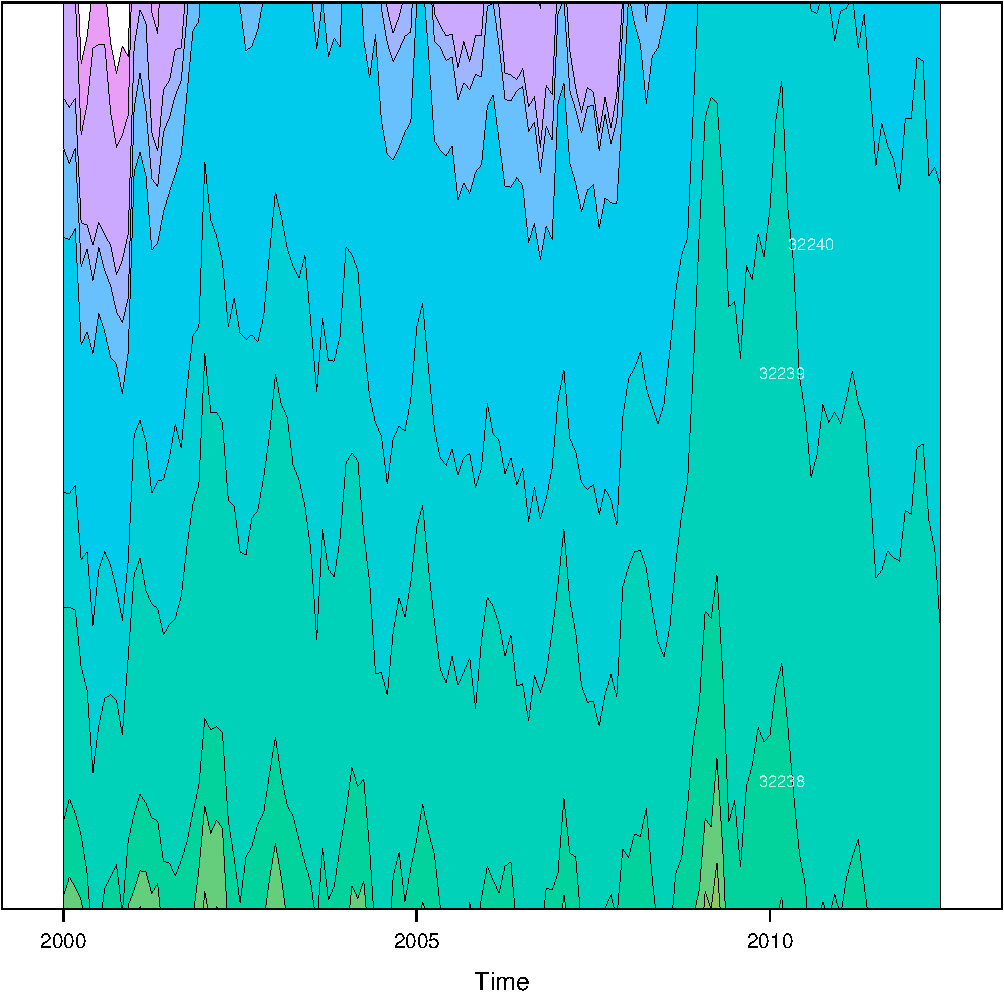
\includegraphics[height=0.45\textheight]{figs/ThemeRiverError.pdf}
\caption{First attempt of ThemeRiver. \label{fig:themeRiverError}}
\end{figure}

The problem is that \texttt{lattice} makes a preliminary estimate of the
window size using a default \texttt{prepanel} function that is unaware of the
internal calculations of our new \texttt{panel.flow} function. The solution
is to define a new \texttt{prepanel.flow} function. 

The input arguments and first lines are the same as in
\texttt{panel.flow}. The output is a list whose elements are the limits for
each axis (\texttt{xlim} and \texttt{ylim}), and the sequence of differences (\texttt{dx}
and \texttt{dy}) that can be used for the aspect and banking
calculations. 

The limits of the x-axis are defined with the range of the time index,
while the limits of the y-axis are calculated with the minimum of the
first column of \texttt{yCumSum} (the origin line) and with the maximum of
its last column (the upper line of the cumulative sum).

\lstset{language=r,label= ,caption= ,captionpos=b,numbers=none}
\begin{lstlisting}
  prepanel.flow <- function(x, y, groups, origin,...){
    dat <- data.frame(x=x, y=y, groups=groups)
    nVars <- nlevels(groups)
    groupLevels <- levels(groups)
    yWide <- unstack(dat, y~groups)
    if (origin=='themeRiver') origin= -1/2*rowSums(yWide)
    else origin=0
    yWide <- cbind(origin=origin, yWide)
    yCumSum <- t(apply(yWide, 1, cumsum))
  
    list(xlim=range(x),
         ylim=c(min(yCumSum[,1]), max(yCumSum[,nVars+1])),
         dx=diff(x),
         dy=diff(c(yCumSum[,-1])))
  }
\end{lstlisting}

\subsection{Interactive \label{sec:interactive}}
\label{sec:orge90985f}

\lstset{language=r,label= ,caption= ,captionpos=b,numbers=none}
\begin{lstlisting}
## remotes::install_github("hrbrmstr/streamgraph")
library(streamgraph)
library(reshape2)
\end{lstlisting}

\lstset{language=r,label= ,caption= ,captionpos=b,numbers=none}
\begin{lstlisting}
unemployDF <- as.data.frame(unemployUSA)

unemployDF$time <- as.Date(index(unemployUSA))

unemployDF <- melt(unemployDF, id.vars = 'time')
\end{lstlisting}

\lstset{language=r,label= ,caption= ,captionpos=b,numbers=none}
\begin{lstlisting}
streamgraph(unemployDF,
            key = "variable",
            value = "value",
            date = "time") %>%
    sg_axis_x(1, "year", "%Y") %>%
    sg_fill_brewer("Set1")
\end{lstlisting}


\chapter{Time as a Conditioning or Grouping Variable}
\label{cha:timeGroupFactor}

In Section \ref{sec:differentVariables} we learned to display the time
evolution of multiple time series with different scales. But, what if
instead of displaying the time evolution we want to confront the
variables between them? Section \ref{SEC:groupVariable} proposes the
scatterplot matrix solution with time as a grouping variable. Section
\ref{SEC:conditionVariable} uses an enhanced scatterplot with time as
a conditioning variable. Section \ref{SEC:hexbin} includes a
digression about the hexagonal binning for large datasets.


\section{Scatterplot Matrix: Time as a Grouping Variable \label{SEC:groupVariable}}
\label{sec:org74c8961}

The scatterplot matrices are based on the technique of small multiples
\cite{Tufte1990}: small, thumbnail-sized representations of multiple
images displayed all at once, which allows the reader to immediately,
and in parallel, compare the inter-frame differences.  A scatterplot
matrix is a display of all pairwise bivariate scatterplots arranged in
a \(p \times p\) matrix for \(p\) variables. Each subplot shows the
relation between the pair of variables at the intersection of the row
and column indicated by the variable names in the diagonal panels
\cite{Friendly.Denis2005}.

This graphical tool is implemented in the \texttt{splom} function. The
following code displays the relation between the set of
meteorological variables using a sequential palette from the
ColorBrewer catalog (\texttt{RbBu}, with black added to complete a
twelve-color palette) to encode the month. The order of colors of
this palette is chosen in order to display summer months with
intense colors and to distinguish between the first and second
half of the year with red and blue, respectively (Figure
\ref{fig:aranjuezSplom}).

\index{splom@\texttt{splom}}


\lstset{language=r,label= ,caption= ,captionpos=b,numbers=none}
\begin{lstlisting}
load('data/aranjuez.RData')
aranjuezDF <- as.data.frame(aranjuez)
aranjuezDF$Month <- format(index(aranjuez), '%m')
\end{lstlisting}

\lstset{language=r,label= ,caption= ,captionpos=b,numbers=none}
\begin{lstlisting}
## Red-Blue palette with black added (12 colors)
colors <- c(brewer.pal(n=11, 'RdBu'), '#000000')
## Rearrange according to months (darkest for summer)
colors <- colors[c(6:1, 12:7)]
\end{lstlisting}

\lstset{language=r,label= ,caption= ,captionpos=b,numbers=none}
\begin{lstlisting}
splom(~ aranjuezDF, 
      groups = aranjuezDF$Month,
      auto.key = list(space = 'right', 
                    title = 'Month', cex.title = 1),
      pscale = 0, varname.cex = 0.7, xlab = '',
      par.settings = custom.theme(symbol = colors,
                                pch = 19),
      cex = 0.3, alpha = 0.1)
\end{lstlisting}

\begin{figure}[htbp]
\centering
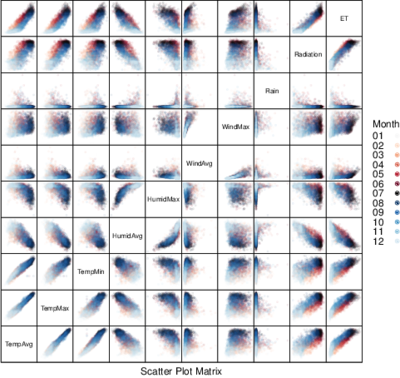
\includegraphics[width=.9\linewidth]{figs/aranjuezSplom.png}
\caption{Scatter plot matrix of the collection of meteorological time series of the Aranjuez station. \label{fig:aranjuezSplom}}
\end{figure}

A bit of interactivity can be added to this plot with the
identification of some points. This task is easy with
\texttt{panel.link.splom}. The points are selected via mouse clicks (and
highlighted in green). Clicks other than left-clicks terminate the
procedure. The output of this function is the index of chosen
points.

\index{panel.link.splom@\texttt{panel.link.splom}}
\index{trellis.focus@\texttt{trellis.focus}}

\lstset{language=r,label= ,caption= ,captionpos=b,numbers=none}
\begin{lstlisting}
trellis.focus('panel', 1, 1)
idx <- panel.link.splom(pch=13, cex=0.6, col='green')
aranjuez[idx,]
\end{lstlisting}

The \texttt{ggplot2} version of Figure \ref{fig:aranjuezSplom} is produced
thanks to the \texttt{ggpairs} function provided by the \texttt{GGally} package.

\index{ggpairs@\texttt{ggpairs}}
\index{Packages!GGally@\texttt{GGally}}

\lstset{language=r,label= ,caption= ,captionpos=b,numbers=none}
\begin{lstlisting}
library(GGally)

ggpairs(aranjuezDF,
        columns = 1:10, ## Do not include "Month"
        upper = list(continuous = "points"),
        mapping = aes(colour = Month, alpha = 0.1))
\end{lstlisting}

Let's explore Figure \ref{fig:aranjuezSplom}. For example,
\begin{itemize}
\item The highest values of ambient temperature (average, maximum, and
minimum), solar radiation, and evotranspiration can be found during
the summer.
\item These variables are almost linearly related. The relation between
radiation and temperature is different during both halves of the
year (red and blue regions can be easily distinguished).
\item The humidity reaches its highest values during winter without
appreciable differences between the first and second half of the
year. The temperature and humidity may be related with an
exponential function.
\end{itemize}

\subsection{Hexagonal Binning \label{SEC:hexbin}}
\label{sec:org7703232}

For large datasets, the display of a large number of points in a
scatterplot produces hidden point density, long computation times,
and slow displays. These problems can be circumvented with the
estimation and representation of points densities.  A common
encoding uses gray scales, pseudo colors or partial
transparency. An improved scheme encodes density as the size of
hexagon symbols inscribed within hexagonal binning regions
\cite{Carr.Littlefield.ea1987}.

The \texttt{hexbin} package \cite{Carr.Lewin-Koh.ea2013} includes several
functions for hexagonal binning.  The \texttt{panel.hexbinplot} is a good
substitute for the default panel function. In addition, our first
attempt with \texttt{splom} can be improved with several modifications
(Figure \ref{fig:aranjuezSplomHexbin}):
\begin{itemize}
\item The scale's ticks and labels are suppressed with \texttt{pscale=0}.
\item The panels of the lower part of the matrix (\texttt{lower.panel}) will
include a locally weighted scatterplot smoothing (loess) with
\texttt{panel.loess}.
\item The diagonal panels (\texttt{diag.panel}) will display the kernel
density estimate of each variable. The \texttt{density} function
computes this estimate. The result is adjusted to the panel
limits (calculated with \texttt{current.panel.limits}). The kernel
density is plotted with \texttt{panel.lines} and the \texttt{diag.panel.splom}
function completes the content of each diagonal panel.
\item The point density is encoded with the palette \texttt{BTC} (ligther
colors for high density values and darker colors for almost
empty regions, with a gradient of blue hues for intermediate values).
\end{itemize}


\index{Packages!hexbin@\texttt{hexbin}}
\index{panel.hexbinplot@\texttt{panel.hexbinplot}}
\index{panel.loess@\texttt{panel.loess}}
\index{diag.panel.splom@\texttt{diag.panel.splom}}
\index{current.panel.limits@\texttt{current.panel.limits}}
\index{Panel function}


\lstset{language=r,label= ,caption= ,captionpos=b,numbers=none}
\begin{lstlisting}
library(hexbin)
  
splom(~as.data.frame(aranjuez),
      panel = panel.hexbinplot,
      colramp = BTC,
      diag.panel = function(x, ...){
          yrng <- current.panel.limits()$ylim
          d <- density(x, na.rm = TRUE)
          d$y <- with(d, yrng[1] + 0.95 * diff(yrng) * y / max(y))
          panel.lines(d)
          diag.panel.splom(x, ...)
      },
      lower.panel = function(x, y, ...){
          panel.hexbinplot(x, y, ...)
          panel.loess(x, y, ..., col = 'red')
      },
      xlab = '',
      pscale = 0, varname.cex = 0.7)
\end{lstlisting}

\begin{figure}[htbp]
\centering
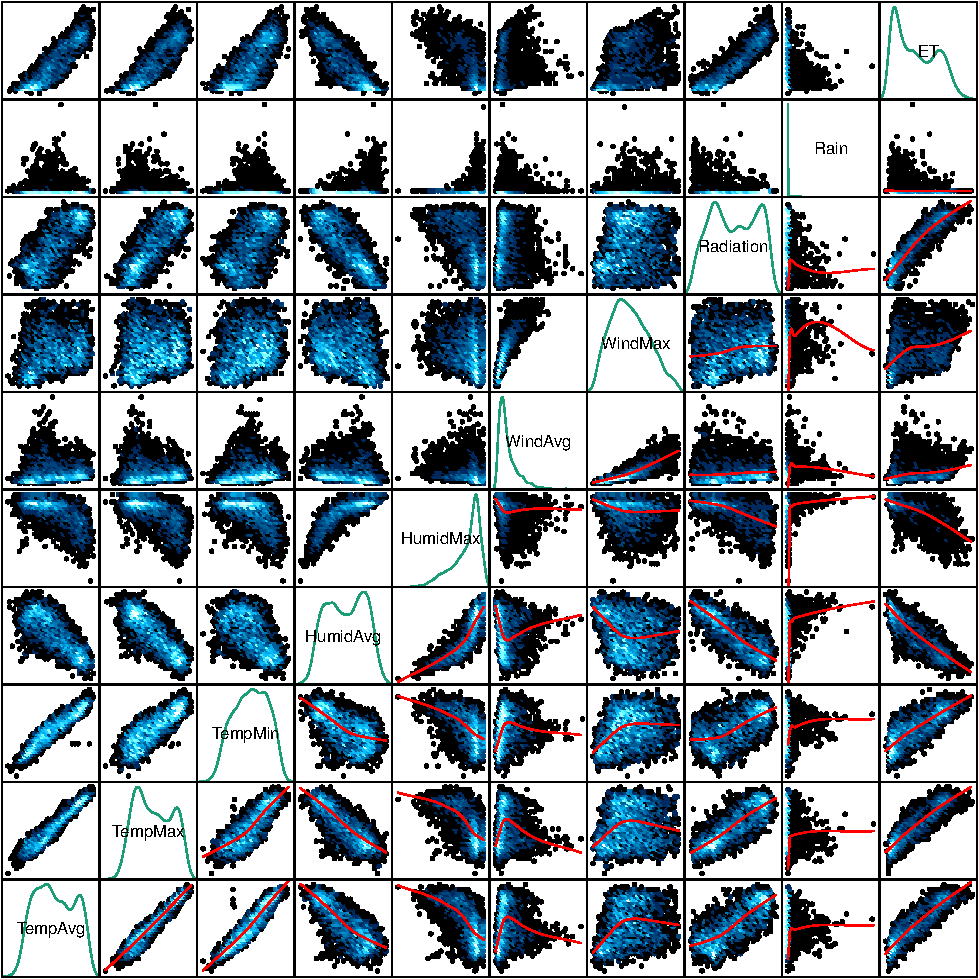
\includegraphics[width=.9\linewidth]{figs/aranjuezSplomHexbin.pdf}
\caption{Scatterplot matrix of the collection of meteorological time series of the Aranjuez station using hexagonal binning. \label{fig:aranjuezSplomHexbin}}
\end{figure}

A drawback of the matrix of scatterplots with hexagonal binning is
that each panel is drawn independently, so it is impossible to compute
a common color key for all of them. In other words, two cells with
exactly the same color in different panels encode different point
densities.

It is possible to display a reduced set of variables against another
one and generate a common color key using the \texttt{hexbinplot}
function. First, the dataset must be reshaped from the wide format
(one colum for each variable) to the long format (only one column for
the temperature values with one row for each observation). This task
is easily accomplished with the \texttt{melt} function included in the
\texttt{reshape2} package.

\index{melt\texttt{melt}}
\index{Packages!reshape2@\texttt{reshape2}}

\lstset{language=r,label= ,caption= ,captionpos=b,numbers=none}
\begin{lstlisting}
library(reshape2)

aranjuezRshp <- melt(aranjuezDF,
                     measure.vars = c('TempMax',
                                      'TempAvg',
                                      'TempMin'),
                     variable.name = 'Statistic',
                     value.name = 'Temperature')
\end{lstlisting}


\lstset{language=r,label= ,caption= ,captionpos=b,numbers=none}
\begin{lstlisting}
head(aranjuezRshp)
\end{lstlisting}

The \texttt{hexbinplot} displays this dataset with a different panel for
each type of temperature (average, maximum, and minimum) but with a
common color key encoding the point density (Figure
\ref{fig:aranjuezHexbin}). Now, two cells with the same color in
different panels encode the same value. 

\index{hexbinplot@\texttt{hexbinplot}}
\index{Panel function}

\lstset{language=r,label= ,caption= ,captionpos=b,numbers=none}
\begin{lstlisting}
hexbinplot(Radiation ~ Temperature | Statistic,
           data = aranjuezRshp,
           layout = c(1, 3),
           colramp = BTC) +
    layer(panel.loess(..., col = 'red'))
\end{lstlisting}

\begin{figure}[htbp]
\centering
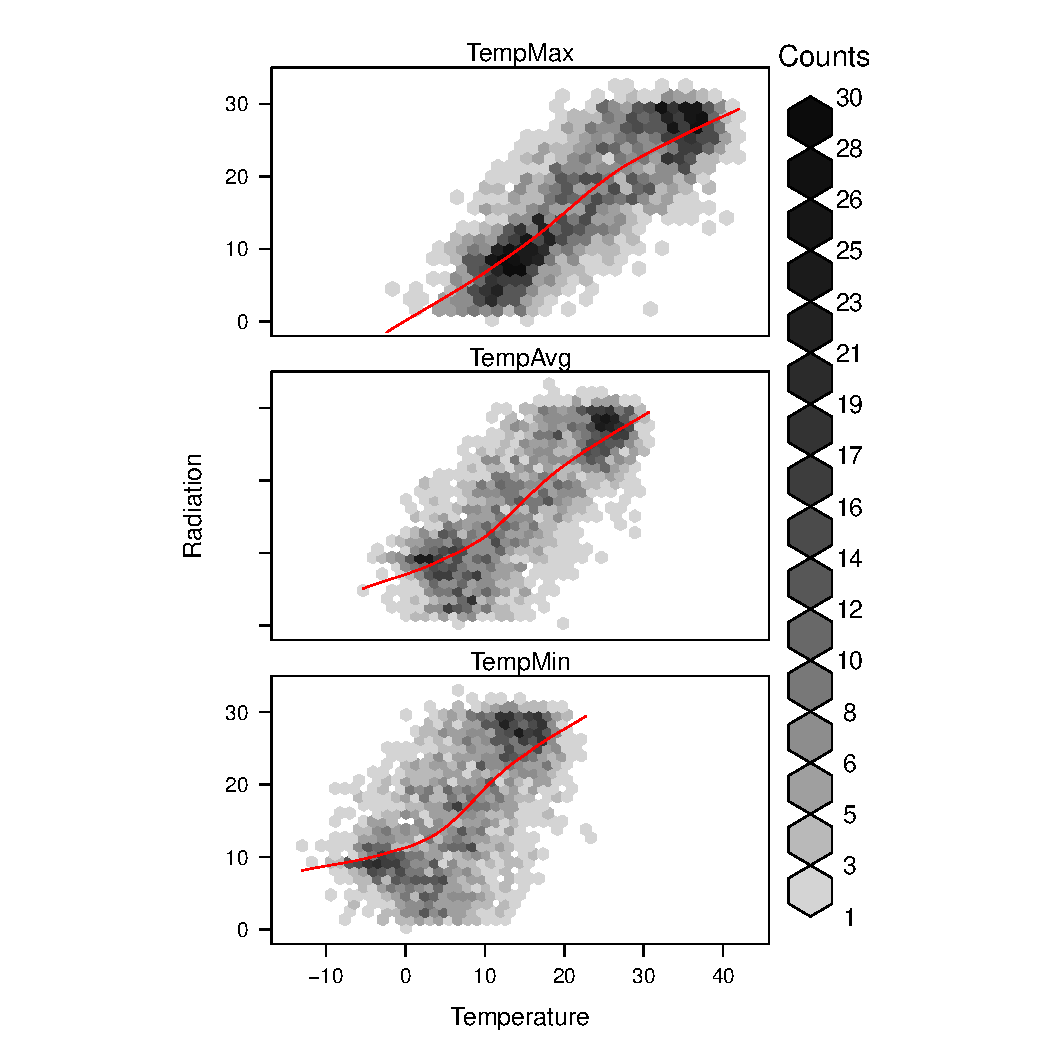
\includegraphics[width=.9\linewidth]{figs/aranjuezHexbinplot.pdf}
\caption{Scatterplot with hexagonal binning of temperature versus solar radiation using data of the Aranjuez station (\texttt{lattice} version). \label{fig:aranjuezHexbin}}
\end{figure}

The ggplot2 version is based on the \texttt{stat\_binhex} function.
\lstset{language=r,label= ,caption= ,captionpos=b,numbers=none}
\begin{lstlisting}
ggplot(data = aranjuezRshp,
       aes(Temperature, Radiation)) +
    stat_binhex(ncol = 1) + 
    stat_smooth(se = FALSE, method = 'loess', col = 'red') +
    facet_wrap(~ Statistic, ncol = 1) +
    theme_bw()
\end{lstlisting}

\section{Scatterplot with Time as a Conditioning Variable \label{SEC:conditionVariable}}
\label{sec:orgc5550a4}

After discussing the hexagonal binning, let's recover the time
variable. Figure \ref{fig:aranjuezSplom} uses colors to encode
months. Instead, we will now display separate scatterplots with a
panel for each month. In addition, the statistic type (average,
maximum, minimum) is included as an additional conditioning variable.

This matrix of panels can be displayed with \texttt{ggplot} using
\texttt{facet\_grid}. The code of Figure \ref{fig:aranjuezFacetGrid} uses partial
transparency to cope with overplotting, small horizontal and vertical
segments (\texttt{geom\_rug}) to display points density on both variables, and
a smooth line in each panel.
\lstset{language=r,label= ,caption= ,captionpos=b,numbers=none}
\begin{lstlisting}
ggplot(data = aranjuezRshp, aes(Radiation, Temperature)) +
    facet_grid(Statistic ~ month) +
    geom_point(col = 'skyblue4', pch = 19, cex = 0.5, alpha = 0.3) +
    geom_rug() +
    stat_smooth(se = FALSE, method = 'loess', col = 'indianred1', lwd = 1.2) +
    theme_bw()
\end{lstlisting}

\begin{figure}[htbp]
\centering
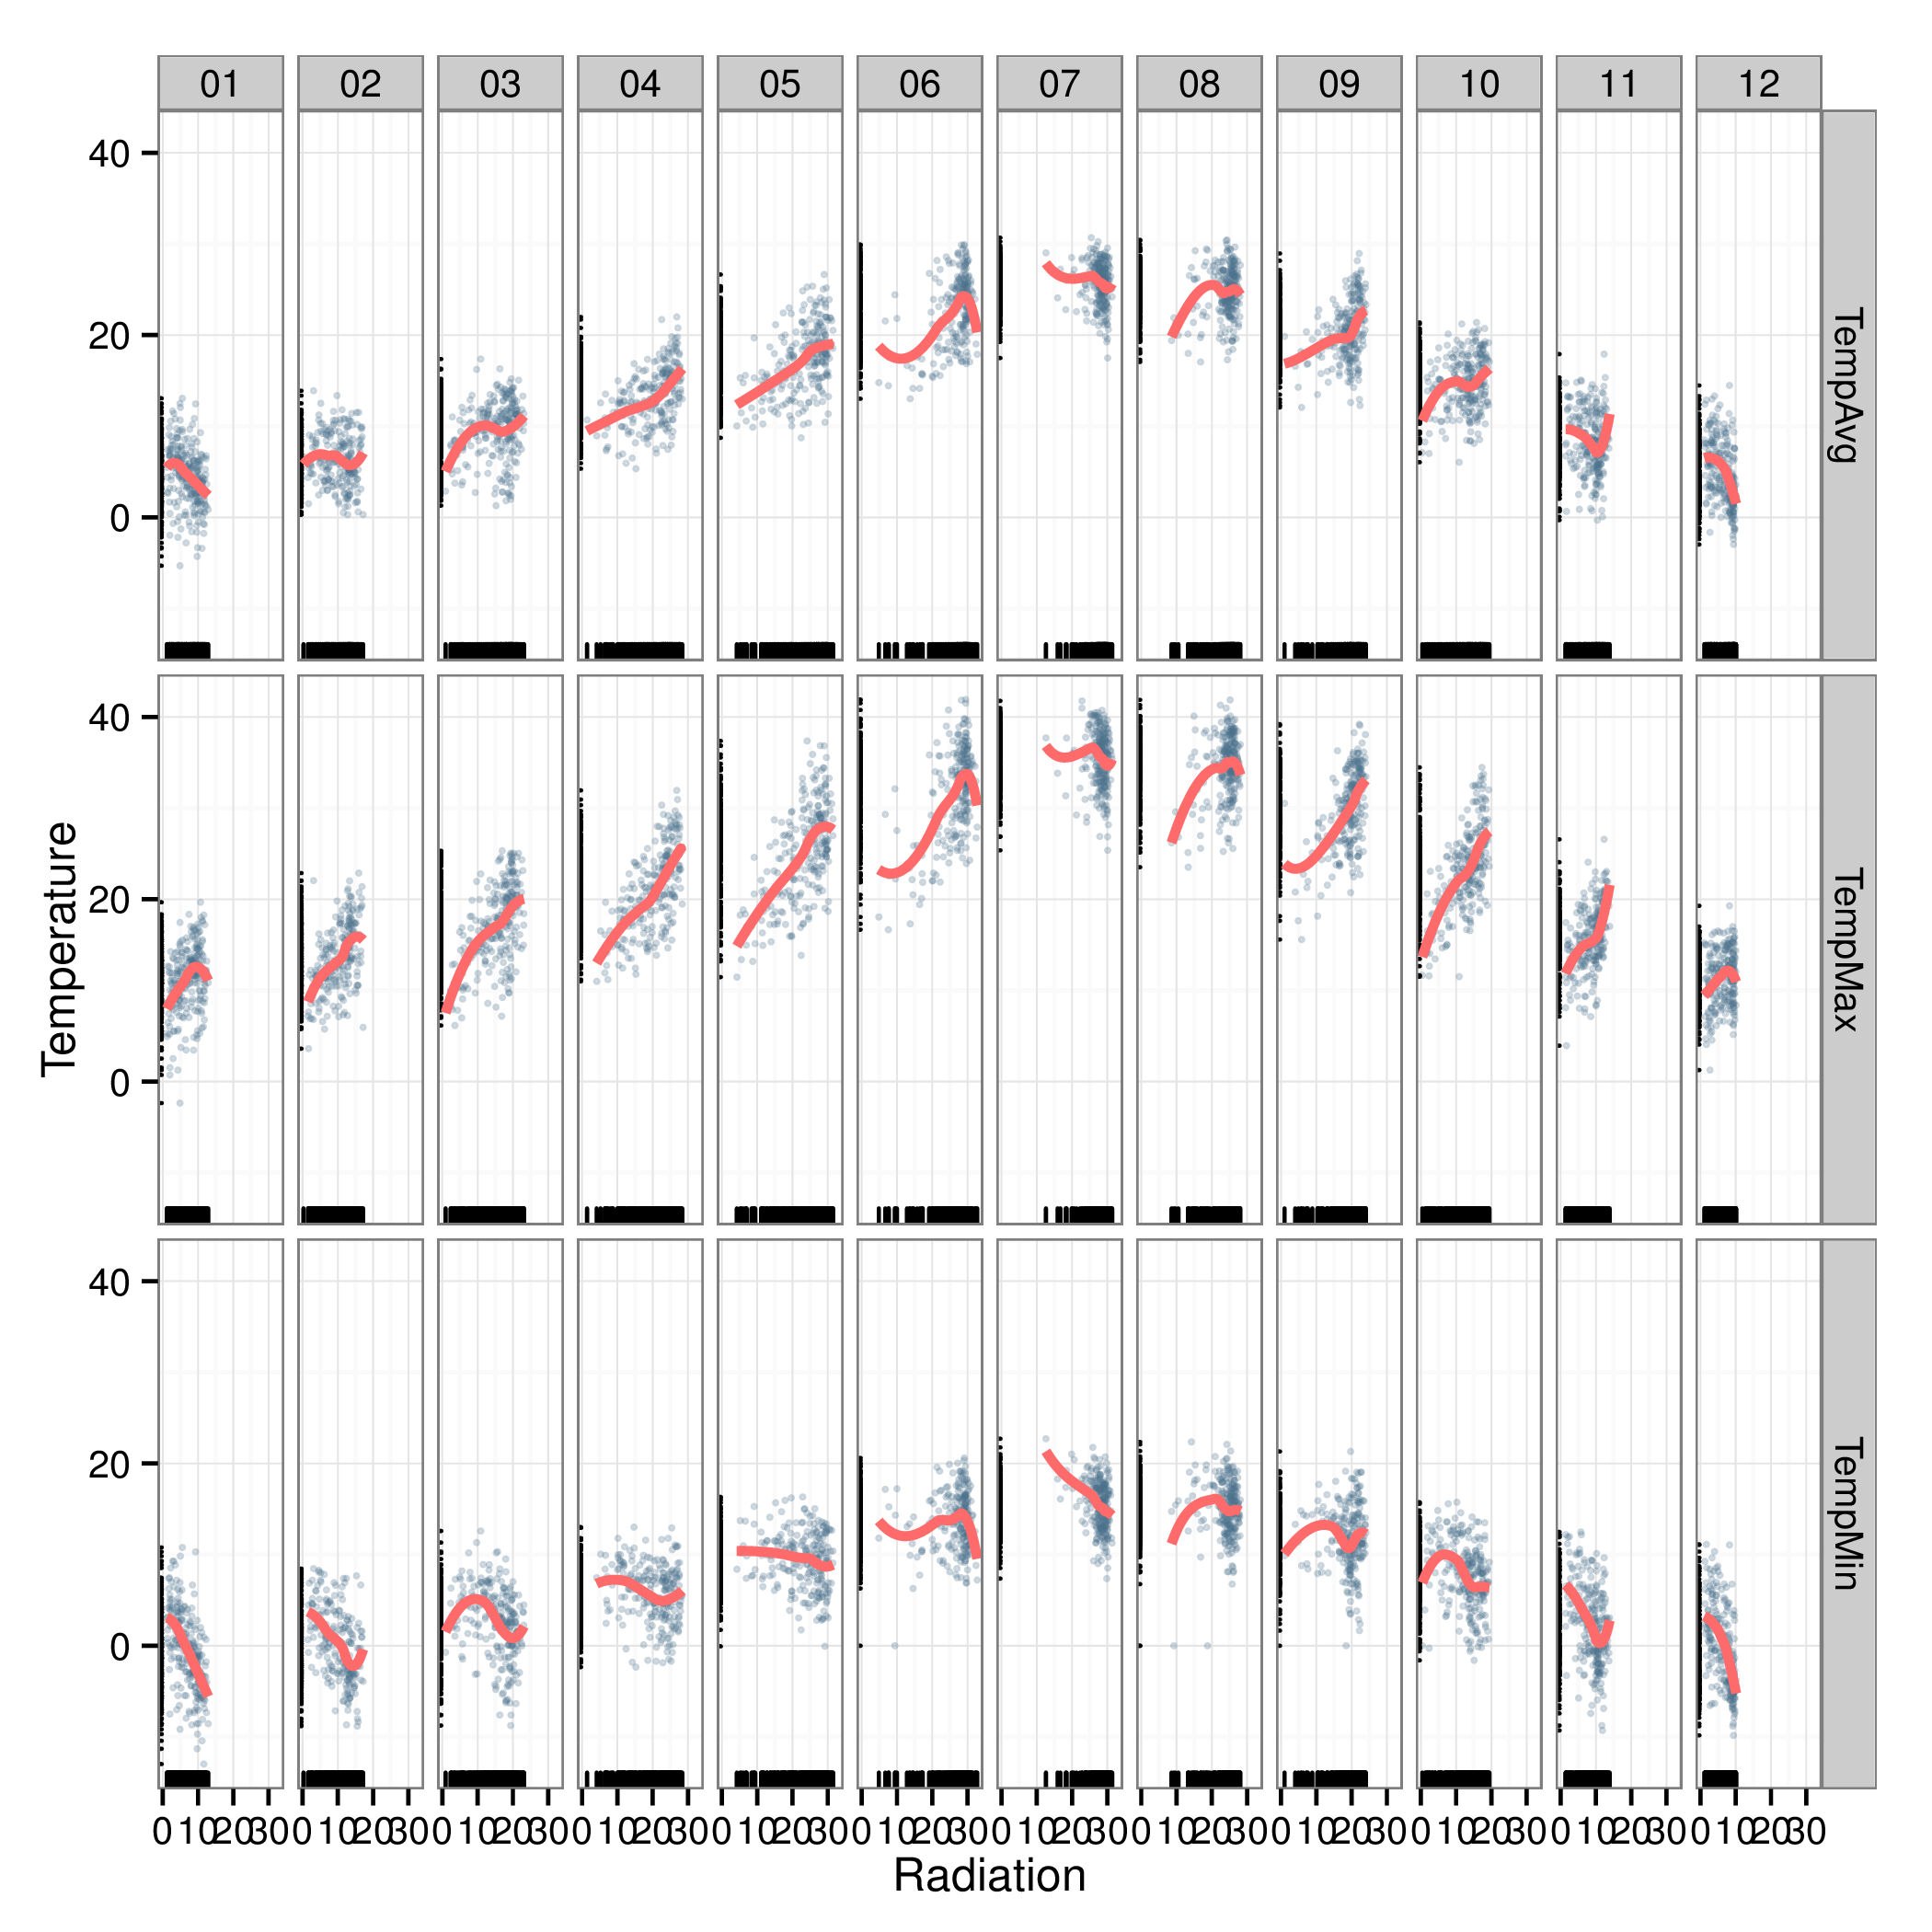
\includegraphics[width=.9\linewidth]{figs/aranjuezFacetGrid.png}
\caption{Scatterplot of temperature versus solar radiation for each month using data of the Aranjuez station (\texttt{ggplot2} version). \label{fig:aranjuezFacetGrid}}
\end{figure}

The version with \texttt{lattice} needs the \texttt{useOuterStrips} function from
the \texttt{latticeExtra} package, which prints the names of the conditioning
variables on the top and left outer margins (Figure
 \ref{fig:aranjuezOuterStrips}).

\index{useOuterStrips@\texttt{useOuterStrips}}
\index{panel.rug@\texttt{panel.rug}}
\index{panel.loess@\texttt{panel.loess}}
\index{Packages!latticeExtra@\texttt{latticeExtra}}

\lstset{language=r,label= ,caption= ,captionpos=b,numbers=none}
\begin{lstlisting}
useOuterStrips(xyplot(Temperature ~ Radiation | month * Statistic,
                      data = aranjuezRshp,
                      between = list(x = 0),
                      col = 'skyblue4', pch = 19,
                      cex = 0.5, alpha = 0.3)) +
    layer({
        panel.rug(..., col.line = 'indianred1', end = 0.05, alpha = 0.6)
        panel.loess(..., col = 'indianred1', lwd = 1.5, alpha = 1)
    })
\end{lstlisting}

\begin{figure}[htbp]
\centering
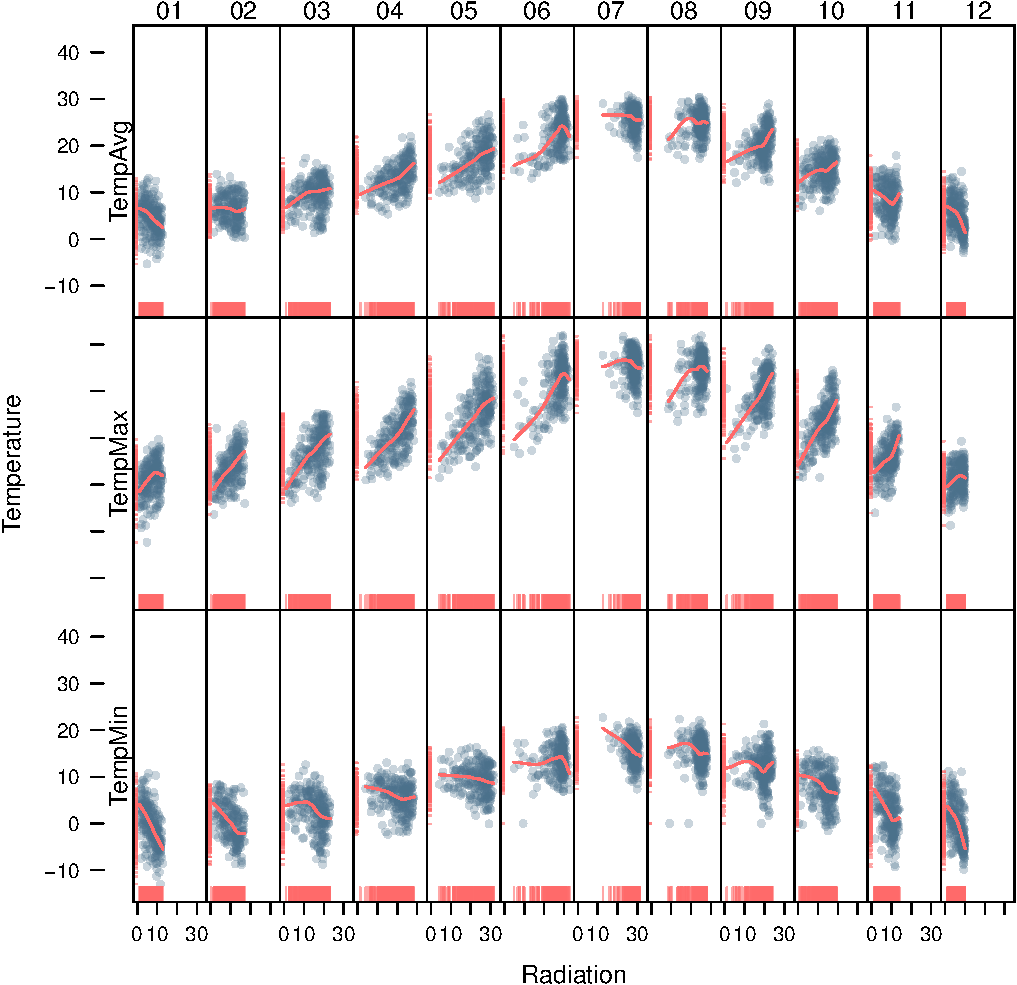
\includegraphics[width=.9\linewidth]{figs/aranjuezOuterStrips.pdf}
\caption{Scatterplot of temperature versus solar radiation for each month using data of the Aranjuez station (lattice version). \label{fig:aranjuezOuterStrips}}
\end{figure}

These figures show the typical seasonal behavior of solar radiation
and ambient temperature. Additionally, it displays in more detail the
same relations between radiation and temperature already discussed
with Figure \ref{fig:aranjuezHexbin}.


\chapter{Time as a Complementary Variable}
\label{cha:timeComplementary}

Gapminder\footnote{\url{http://www.gapminder.org/}} is an independent
foundation based in Stockholm, Sweden. Its mission is ``to debunk
devastating myths about the world by offering free access to a
fact-based world view.'' They provide free online tools, data, and
videos ``to better understand the changing world.'' The initial
development of Gapminder was the Trendalyzer software, used by Hans
Rosling in several sequences of his documentary ``The Joy of Stats.''

The information visualization technique used by Trendalyzer is an
interactive bubble chart. By default it shows five variables: two
numeric variables on the vertical and horizontal axes, bubble size and
color, and a time variable that may be manipulated with a slider. The
software uses brushing and linking techniques for displaying the
numeric value of a highlighted country.

This software was acquired by Google\textsuperscript{\textregistered}
in 2007, and is now available as a Motion Chart gadget and as the
Public Data Explorer.

In this chapter, time will be used as a complementary variable which
adds information to a graph where several variables are confronted. We
will illustrate this approach with the evolution of the relationship
between Gross National Income (GNI) and carbon dioxide ($CO_2$)
emissions for a set of countries extracted from the database of the
World Bank Open Data. We will try several solutions to display the
relationship between $CO_2$ emissions and GNI over the years using
time as a complementary variable. The final method will produce an
animated plot resembling the Trendalyzer solution.


\section{Polylines}
\label{sec:org0c565c6}
\lstset{language=r,label= ,caption= ,captionpos=b,numbers=none}
\begin{lstlisting}
load('data/CO2.RData')
\end{lstlisting}

\index{Data!CO2@$CO_2$}
\index{Data!World Bank}

Our first approach is to display the entire data in a panel with a
scatterplot using country names as the grouping factor. Points of each
country are connected with polylines to reveal the time evolution
(Figure \ref{fig:CO2-GNI}).
\lstset{language=r,label= ,caption= ,captionpos=b,numbers=none}
\begin{lstlisting}
## lattice version
xyplot(GNI.capita  ~ CO2.capita, data=CO2data,
       xlab="Carbon dioxide emissions (metric tons per capita)",
       ylab="GNI per capita, PPP (current international $)",
       groups=Country.Name, type='b')
\end{lstlisting}

\begin{figure}[htbp]
\centering
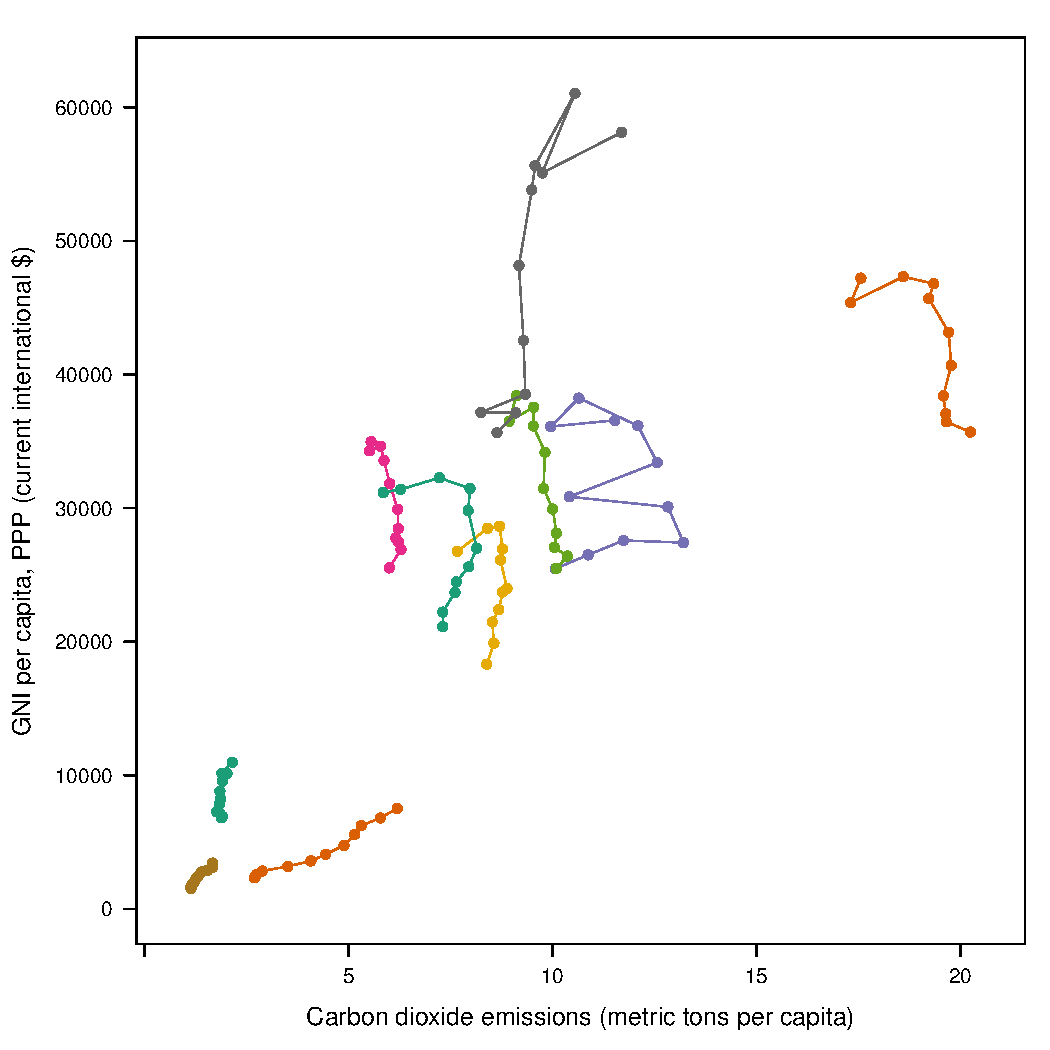
\includegraphics[width=.9\linewidth]{figs/CO2_GNI.pdf}
\caption{GNI per capita versus \(\mathrm{CO_2}\) emissions per capita (\texttt{lattice} version). \label{fig:CO2-GNI}}
\end{figure}

\lstset{language=r,label= ,caption= ,captionpos=b,numbers=none}
\begin{lstlisting}
## ggplot2 version
ggplot(data=CO2data, aes(x=CO2.capita, y=GNI.capita,
                         color=Country.Name)) +
    xlab("Carbon dioxide emissions (metric tons per capita)") +
    ylab("GNI per capita, PPP (current international $)") +
    geom_point() + geom_path() + theme_bw()
\end{lstlisting}

Three improvements can be added to this graphical result: 
\begin{enumerate}
\item Define a better palette to enhance visual discrimination between
countries.
\item Display time information with labels to show year values.
\item Label each polyline with the country name instead of a legend.
\end{enumerate}

\section{Choosing Colors}
\label{sec:org8e11acd}
The \texttt{Country.Name} categorical variable will be encoded with a
qualitative palette, namely the first five colors of \texttt{Set1}
palette\footnote{\url{http://colorbrewer2.org/}} from the \texttt{RColorBrewer} package
\cite{Neuwirth2011}. Because there are more countries than colors, we
have to repeat some colors to complete the number of levels of the
variable \texttt{Country.Name}. The result is a palette with non-unique
colors, and thus some countries will share the same color. This is not
a problem because the curves will be labeled, and countries with the
same color will be displayed at enough distance.

\index{Packages!RColorBrewer@\texttt{RColorBrewer}}
\index{brewer.pal@\texttt{brewer.pal}}

\lstset{language=r,label= ,caption= ,captionpos=b,numbers=none}
\begin{lstlisting}
library(RColorBrewer)

nCountries <- nlevels(CO2data$Country.Name)
pal <- brewer.pal(n=5, 'Set1')
pal <- rep(pal, length = nCountries)
\end{lstlisting}

Adjacent colors of this palette are chosen to be easily
distinguishable. Therefore, the connection between colors and
countries must be in such a way that nearby lines are encoded
with adjacent colors of the palette.

A simple approach is to calculate the annual average of the
variable to be represented along the x-axis (\texttt{CO2.capita}), and
extract colors from the palette according to the order of this
value.  

\index{aggregate@\texttt{aggregate}}

\lstset{language=r,label= ,caption= ,captionpos=b,numbers=none}
\begin{lstlisting}
## Rank of average values of CO2 per capita
CO2mean <- aggregate(CO2.capita ~ Country.Name, data=CO2data, FUN=mean)
palOrdered <- pal[rank(CO2mean$CO2.capita)]  
\end{lstlisting}

A more sophisticated solution is to use the ordered results of a
hierarchical clustering of the time evolution of the \(\mathrm{CO_2}\) per capita
values (Figure \ref{fig:hclustCO2}). The data is extracted from the
original \(\mathrm{CO_2}\) \texttt{data.frame}.  

\index{hclust@\texttt{hclust}}

\lstset{language=r,label= ,caption= ,captionpos=b,numbers=none}
\begin{lstlisting}
CO2capita <- CO2data[, c('Country.Name',
                         'Year',
                         'CO2.capita')]
CO2capita <- reshape(CO2capita,
                     idvar='Country.Name',
                     timevar='Year',
                     direction='wide')
hCO2 <- hclust(dist(CO2capita[, -1]))

oldpar <- par(mar=c(0, 2, 0, 0) + .1)
plot(hCO2, labels=CO2capita$Country.Name,
     xlab='', ylab='', sub='', main='')
par(oldpar)
\end{lstlisting}

\begin{figure}[htbp]
\centering
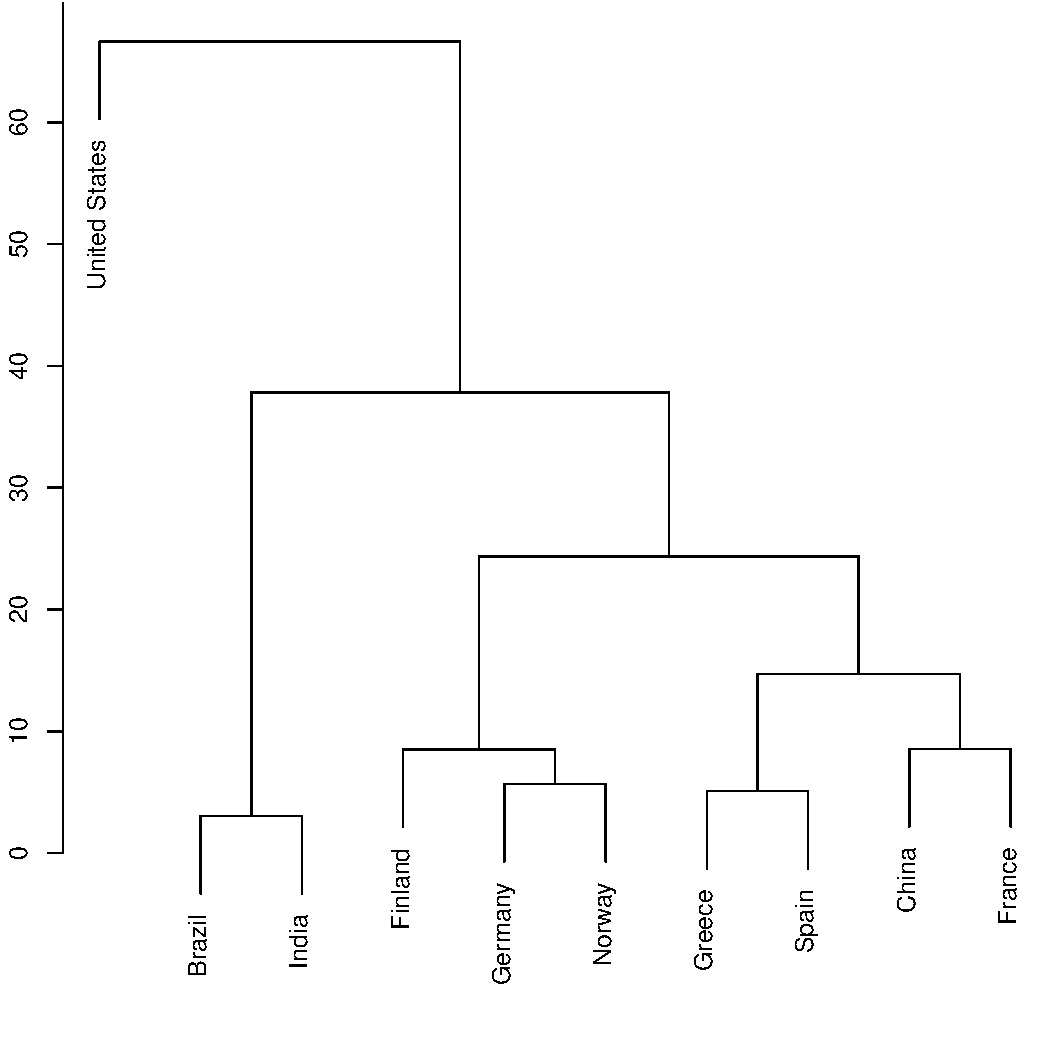
\includegraphics[width=.9\linewidth]{figs/hclust.pdf}
\caption{Hierarchical clustering of the time evolution of \(\mathrm{CO_2}\) per capita values. \label{fig:hclustCO2}}
\end{figure}


The colors of the palette are assigned to each country with \texttt{match},
which returns a vector of the positions of the matches of the country
names in alphabetical order in the country names ordered according to
the hierarchical clustering.
\lstset{language=r,label= ,caption= ,captionpos=b,numbers=none}
\begin{lstlisting}
idx <- match(levels(CO2data$Country.Name), 
             CO2capita$Country.Name[hCO2$order])
palOrdered <- pal[idx]  
\end{lstlisting}
It must be highlighted that this palette links colors with the levels
of \texttt{Country.Name} (country names in alphabetical order), which is
exactly what the \texttt{groups} argument provides. The following code
produces a curve for each country using different colors to
distinguish them.

\index{simpleTheme@\texttt{simpleTheme}}
\lstset{language=r,label= ,caption= ,captionpos=b,numbers=none}
\begin{lstlisting}
## simpleTheme encapsulates the palette in a new theme for xyplot
myTheme <- simpleTheme(pch=19, cex=0.6, col=palOrdered)

pCO2.capita <- xyplot(GNI.capita  ~ CO2.capita,
                      data = CO2data,
                      xlab = "Carbon dioxide emissions (metric tons per capita)",
                      ylab = "GNI per capita, PPP (current international $)",
                      groups = Country.Name,
                      par.settings = myTheme,
                      type='b')
\end{lstlisting}

\lstset{language=r,label= ,caption= ,captionpos=b,numbers=none}
\begin{lstlisting}
gCO2.capita <- ggplot(data = CO2data,
                      aes(x = CO2.capita,
                          y = GNI.capita,
                          color = Country.Name)) +
    geom_point() + geom_path() +
    scale_color_manual(values=palOrdered, guide=FALSE) +
    xlab('CO2 emissions (metric tons per capita)') +
    ylab('GNI per capita, PPP (current international $)') +
    theme_bw()
\end{lstlisting}

\section{Labels to Show Time Information}
\label{sec:org06fa9e5}
This result can be improved with labels displaying the years to show
the time evolution.  A panel function with \texttt{panel.text} to print the
year labels and \texttt{panel.superpose} to display the lines for each group
is a solution. In the panel function, \texttt{subscripts} is a vector with
the integer indices representing the rows of the \texttt{data.frame} to be
displayed in the panel.

\index{panel.text@\texttt{panel.text}}
\index{subscripts@\texttt{subscripts}}
\index{Panel function}
\index{panel.superpose@\texttt{panel.superpose}}


\lstset{language=r,label= ,caption= ,captionpos=b,numbers=none}
\begin{lstlisting}
xyplot(GNI.capita  ~ CO2.capita,
       data = CO2data
       xlab = "Carbon dioxide emissions (metric tons per capita)",
       ylab = "GNI per capita, PPP (current international $)",
       groups = Country.Name,
       par.settings = myTheme,
       type='b',
       panel = function(x, y, ..., subscripts, groups){
           panel.text(x, y, ...,
                      labels = CO2data$Year[subscripts],
                      pos = 2, cex = 0.5, col = 'gray')
           panel.superpose(x, y, subscripts, groups,...)
       })
\end{lstlisting}

The same result with a clearer code is obtained with the combination
of \texttt{+.trellis}, \texttt{glayer\_} and \texttt{panel.text}. Using \texttt{glayer\_} instead of
\texttt{glayer}, we ensure that the labels are printed below the lines.

\index{Packages!latticeExtra@\texttt{latticeExtra}}
\index{glayer@\texttt{glayer}}
\index{+.trellis@\texttt{+.trellis}}

\lstset{language=r,label= ,caption= ,captionpos=b,numbers=none}
\begin{lstlisting}
pCO2.capita <- pCO2.capita +
    glayer_(panel.text(...,
                       labels = CO2data$Year[subscripts],
                         pos = 2, cex = 0.5, col = 'gray'))
\end{lstlisting}

\lstset{language=r,label= ,caption= ,captionpos=b,numbers=none}
\begin{lstlisting}
gCO2.capita <- gCO2.capita + geom_text(aes(label = Year),
                                       colour = 'gray',
                                       size = 2.5,
                                       hjust = 0, vjust = 0)
  
\end{lstlisting}

\section{Country Names: Positioning Labels}
\label{sec:org7621bb0}
The common solution to link each curve with the group value is to add
a legend. However, a legend can be confusing with too many items. In
addition, the reader must carry out a complex task: Choose the line,
memorize its color, search for it in the legend, and read the country
name.

A better approach is to label each line using nearby text with the
same color encoding. A suitable method is to place the labels
close to the end of each line (Figure
\ref{fig:CO2-GNI-glayer}). Labels are placed with the
\texttt{panel.pointLabel} function from the \texttt{maptools} package. This
function use optimization routines to find locations without
overlaps.

\index{group.value@\texttt{group.value}}
\index{group.number@\texttt{group.number}}

\lstset{language=r,label= ,caption= ,captionpos=b,numbers=none}
\begin{lstlisting}
library(maptools)  
## group.value provides the country name; group.number is the index
## of each country to choose the color from the palette.
pCO2.capita +
    glayer(panel.pointLabel(mean(x), mean(y),
                            labels = group.value,
                            col = palOrdered[group.number],
                            cex = .8,
                            fontface = 2,
                            fontfamily = 'Palatino'))
\end{lstlisting}

\begin{figure}[htbp]
\centering
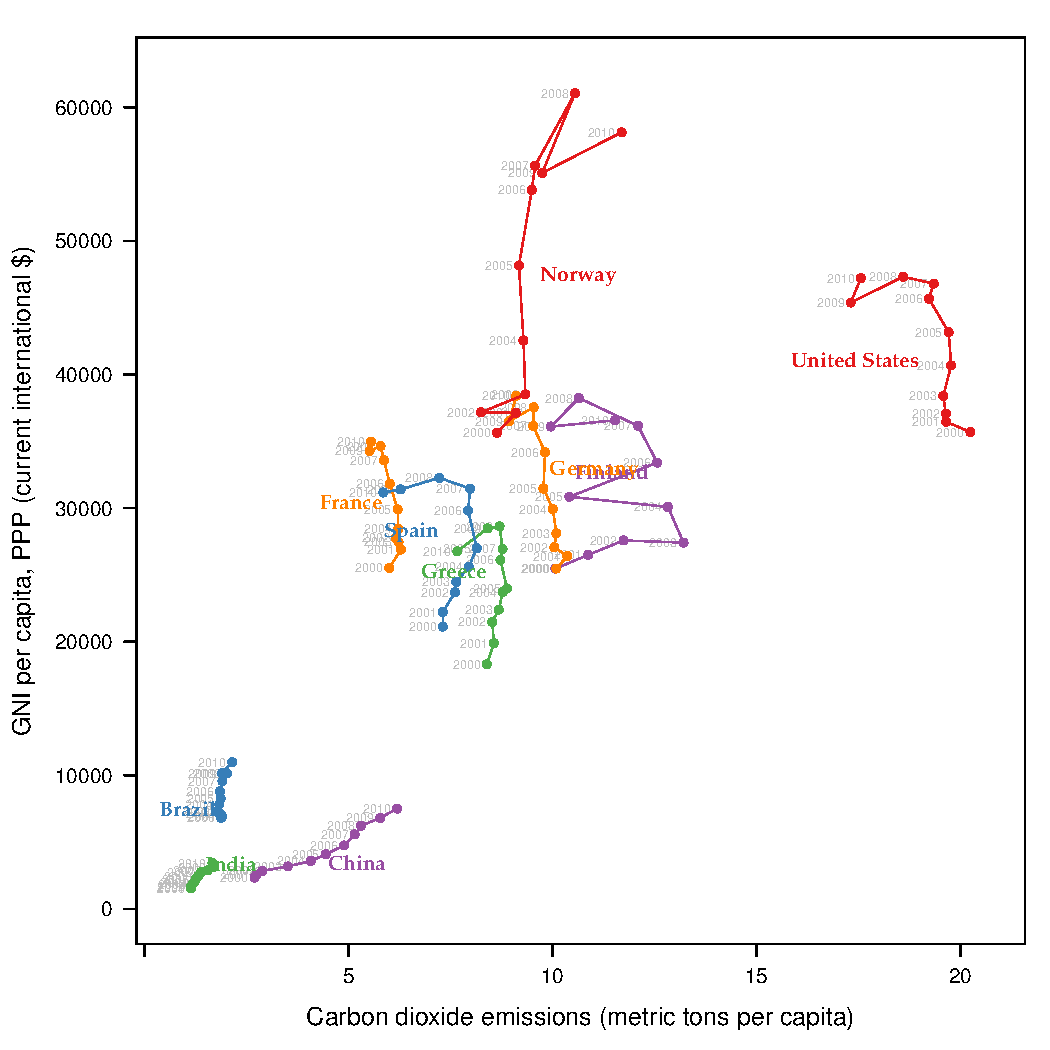
\includegraphics[width=.9\linewidth]{figs/CO2_capita.pdf}
\caption{\(\mathrm{CO_2}\) emissions versus GNI per capita. Labels are placed with \texttt{panel.pointLabel}. \label{fig:CO2-GNI-glayer}}
\end{figure}

However, this solution does not solve the overlapping between labels
and lines. The package \texttt{directlabels} \cite{Hocking2013} includes a
wide repertory of positioning methods to cope with this problem. The
main function, \texttt{direct.label}, is able to determine a suitable method
for each plot, although the user can choose a different method from
the collection or even define a custom method. For the \texttt{pCO2.capita}
object, I have obtained the best results with \texttt{extreme.grid} (Figure
\ref{fig:CO2-GNI-DL}).

\index{Packages!directlabels@\texttt{directlabels}}
\index{direct.label@\texttt{direct.label}}

\lstset{language=r,label= ,caption= ,captionpos=b,numbers=none}
\begin{lstlisting}
library(directlabels)

direct.label(pCO2.capita,
             method = 'extreme.grid')
\end{lstlisting}

\begin{figure}[htbp]
\centering
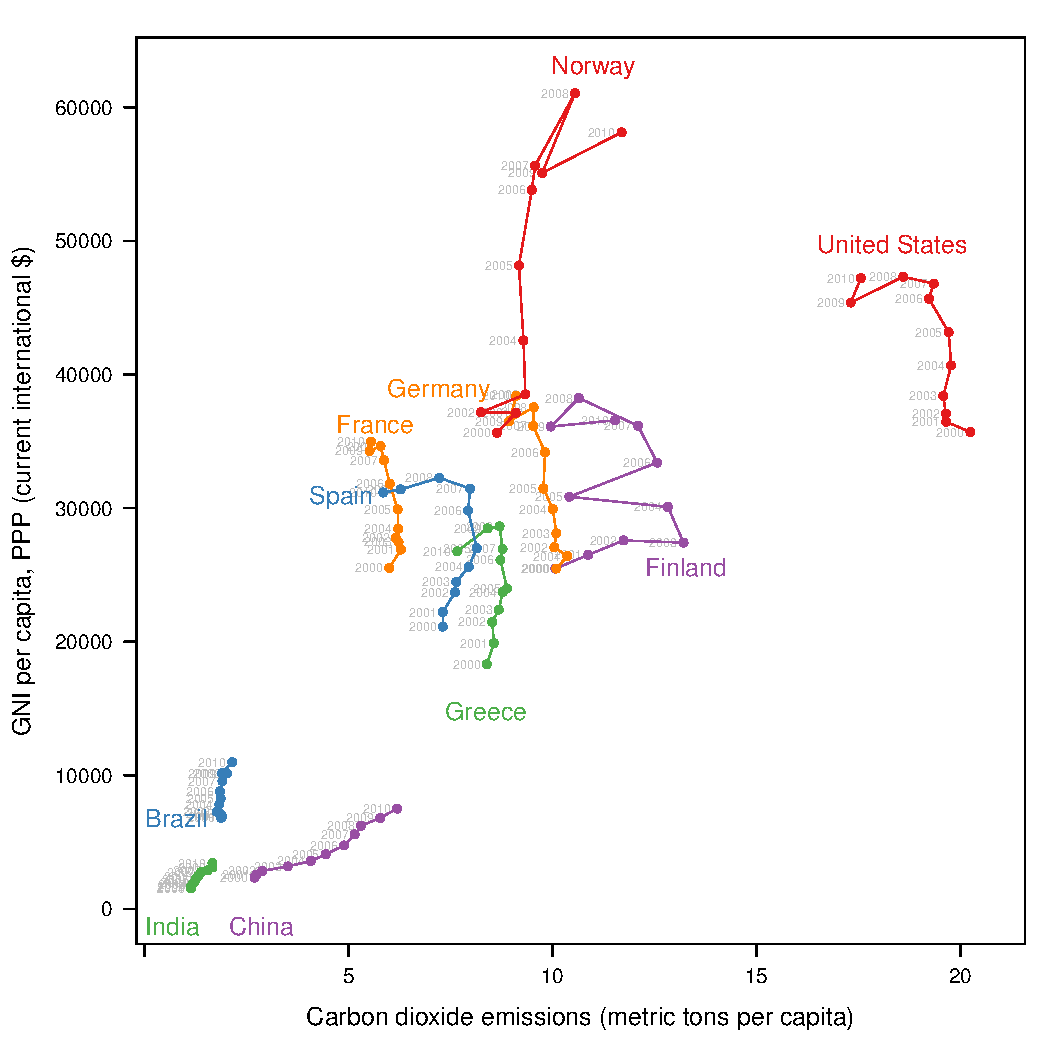
\includegraphics[width=.9\linewidth]{figs/CO2_capitaDL.pdf}
\caption{\(\mathrm{CO_2}\) emissions versus GNI per capita. Labels are placed with the \texttt{extreme.grid} method of the \texttt{directlabels} package. \label{fig:CO2-GNI-DL}}
\end{figure}

\lstset{language=r,label= ,caption= ,captionpos=b,numbers=none}
\begin{lstlisting}
direct.label(gCO2.capita, method='extreme.grid')
\end{lstlisting}

\section{A Panel for Each Year}
\label{sec:orgc320f09}
Time can be used as a conditioning variable (as shown in previous
sections) to display subsets of the data in different panels. Figure
\ref{fig:CO2-GNI-panel} is produced with the same code as in Figure
\ref{fig:CO2-GNI}, now including \texttt{|factor(Year)} in the lattice
version and \texttt{facet\_wrap(\textasciitilde{} Year)} in the \texttt{ggplot2} version.

\lstset{language=r,label= ,caption= ,captionpos=b,numbers=none}
\begin{lstlisting}
xyplot(GNI.capita  ~ CO2.capita | factor(Year),
       data = CO2data,
       xlab = "Carbon dioxide emissions (metric tons per capita)",
       ylab = "GNI per capita, PPP (current international $)",
       groups = Country.Name, type = 'b',
       auto.key = list(space = 'right'))
\end{lstlisting}

\begin{figure}[htbp]
\centering
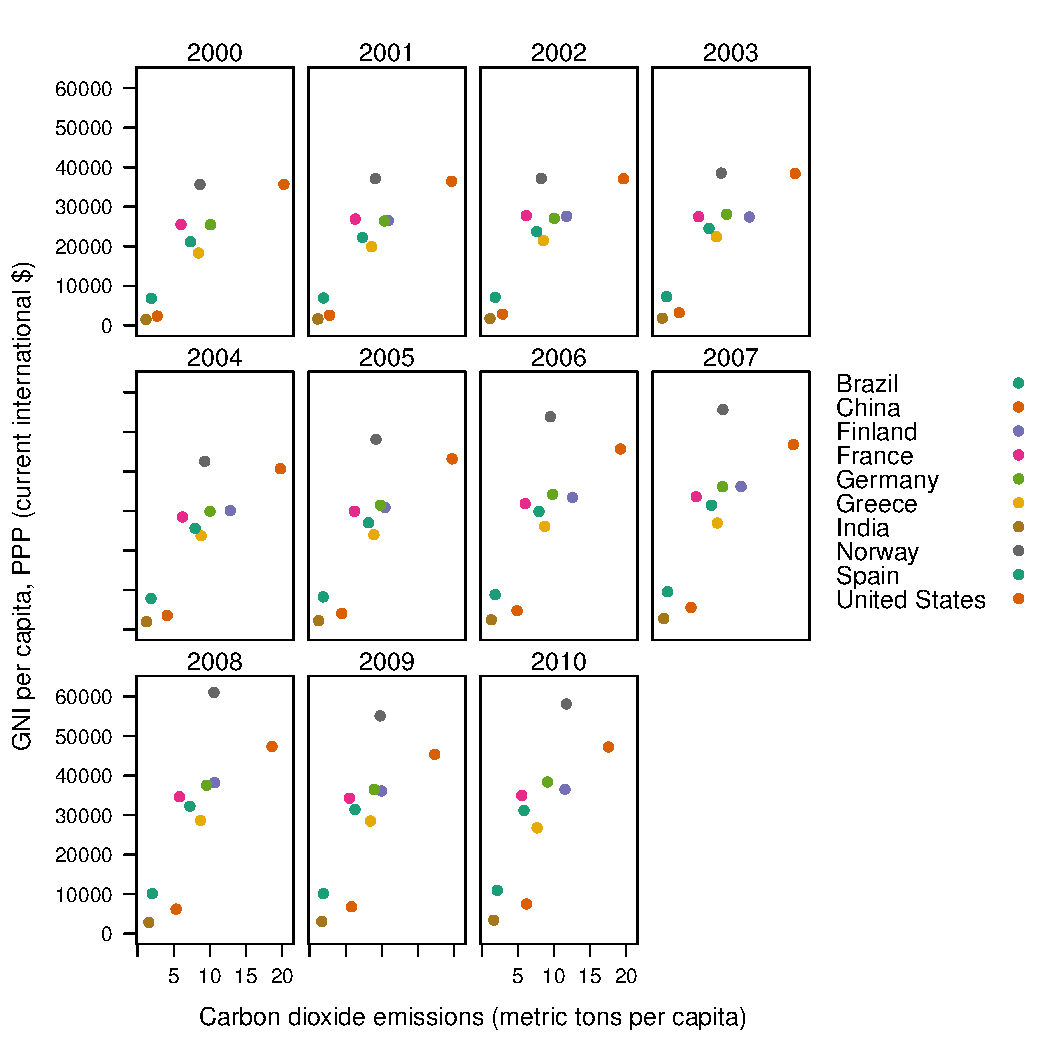
\includegraphics[width=.9\linewidth]{figs/CO2_capita_panel.pdf}
\caption{\(\mathrm{CO_2}\) emissions versus GNI per capita with a panel for each year. \label{fig:CO2-GNI-panel}}
\end{figure}

\lstset{language=r,label= ,caption= ,captionpos=b,numbers=none}
\begin{lstlisting}
ggplot(data = CO2data,
       aes(x = CO2.capita,
           y = GNI.capita,
           colour = Country.Name)) +
    facet_wrap(~ Year) + geom_point(pch = 19) + 
    xlab('CO2 emissions (metric tons per capita)') +
    ylab('GNI per capita, PPP (current international $)') +
    theme_bw()
\end{lstlisting}

Because the grouping variable, \texttt{Country.Name}, has many levels, the
legend is not very useful. Once again, point labeling is recommended
(Figure \ref{fig:CO2-GNI-panel-labels}).

\lstset{language=r,label= ,caption= ,captionpos=b,numbers=none}
\begin{lstlisting}
xyplot(GNI.capita  ~ CO2.capita | factor(Year),
       data = CO2data,
       xlab = "Carbon dioxide emissions (metric tons per capita)",
       ylab = "GNI per capita, PPP (current international $)",
       groups = Country.Name, type = 'b',
       par.settings = myTheme) + 
    glayer(panel.pointLabel(x, y,
                            labels = group.value,
                            col = palOrdered[group.number],
                            cex = 0.7))
\end{lstlisting}

\begin{figure}[htbp]
\centering
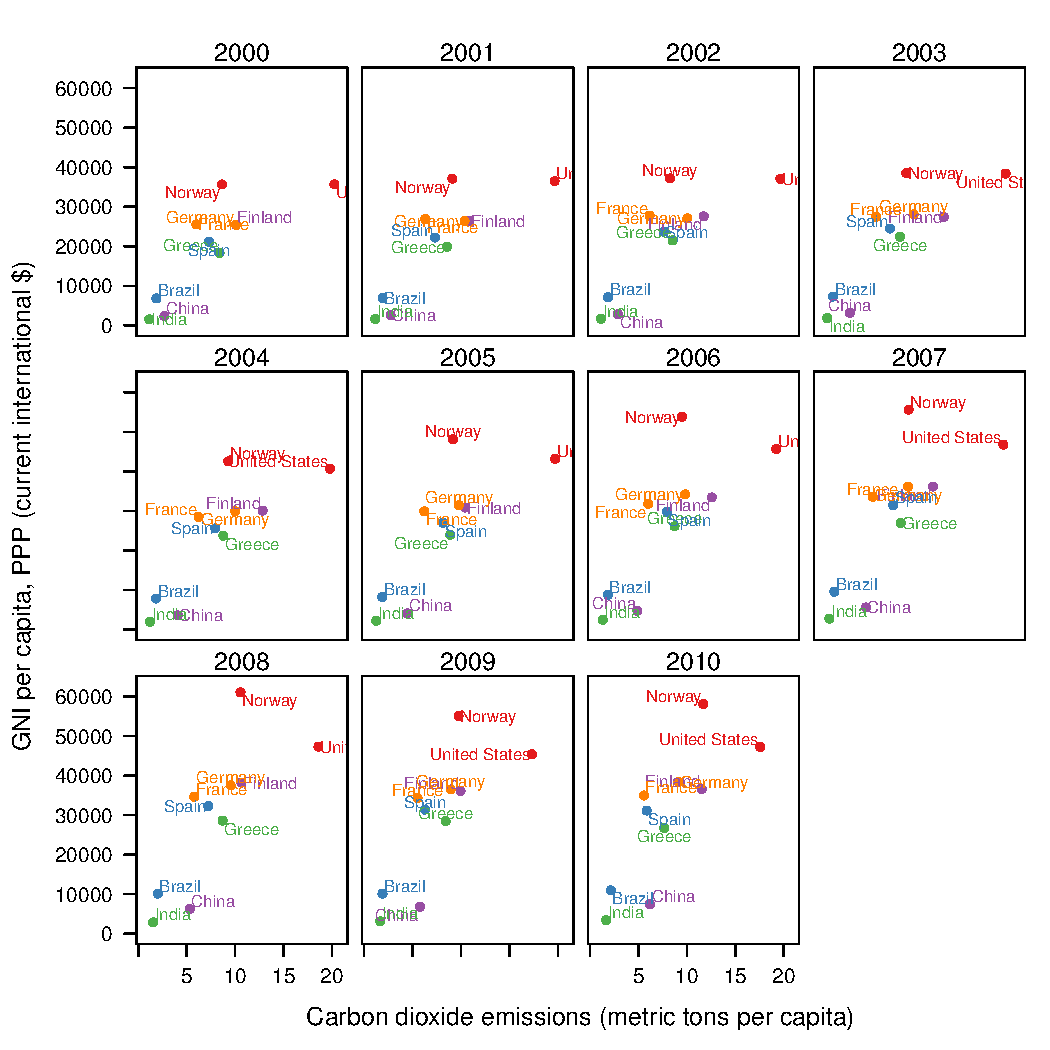
\includegraphics[width=.9\linewidth]{figs/CO2_capita_panel_labels.pdf}
\caption{\(\mathrm{CO_2}\) emissions versus GNI per capita with a panel for each year. \label{fig:CO2-GNI-panel-labels}}
\end{figure}

\subsection{\floweroneleft Using Variable Size to Encode an Additional Variable}
\label{sec:orgdc1eae6}
Instead of using simple points, we can display circles of
different radius to encode a new variable. This new variable is
\texttt{CO2.PPP}, the ratio of \(\mathrm{CO_2}\) emissions to the Gross Domestic
Product with purchasing power parity (PPP) estimations.

To use this numeric variable as an additional grouping factor, its range must be divided into different classes. The typical solution is to use \texttt{cut} to coerce the numeric variable into a \texttt{factor} whose levels correspond to uniform intervals, which could be unrelated to the data distribution. The \texttt{classInt} package \cite{Bivand2013} provides several methods to partition data into classes based on natural groups in the data distribution.

\index{Packages!classInt@\texttt{classInt}}
\index{classIntervals@\texttt{classIntervals}}

\lstset{language=r,label= ,caption= ,captionpos=b,numbers=none}
\begin{lstlisting}
library(classInt)
z <- CO2data$CO2.PPP
intervals <- classIntervals(z, n = 4, style = 'fisher')
\end{lstlisting}

Although the functions of this package are mainly intended to create color palettes for maps, the results can also be associated to point sizes. \texttt{cex.key} defines the sequence of sizes (to be displayed in the legend) associated with each \texttt{CO2.PPP} using the \texttt{findCols} function.
\lstset{language=r,label= ,caption= ,captionpos=b,numbers=none}
\begin{lstlisting}
nInt <- length(intervals$brks) - 1
cex.key <- seq(0.5, 1.8, length = nInt)

idx <- findCols(intervals)
CO2data$cexPoints <- cex.key[idx]
\end{lstlisting}

The graphic will display information on two variables (\texttt{GNI.capita} and \texttt{CO2.capita} in the vertical and horizontal axes, respectively) with a conditioning variable (\texttt{Year}) and two grouping variables (\texttt{Country.Name}, and \texttt{CO2.PPP} through \texttt{cexPoints}) (Figure \ref{fig:CO2pointsGG}).

\lstset{language=r,label= ,caption= ,captionpos=b,numbers=none}
\begin{lstlisting}
ggplot(data = CO2data,
       aes(x = CO2.capita,
           y = GNI.capita,
           colour = Country.Name)) +
    facet_wrap(~ Year) +
    geom_point(aes(size = cexPoints), pch = 19) +
    xlab('Carbon dioxide emissions (metric tons per capita)') +
    ylab('GNI per capita, PPP (current international $)') +
    theme_bw()
\end{lstlisting}

\begin{figure}[htbp]
\centering
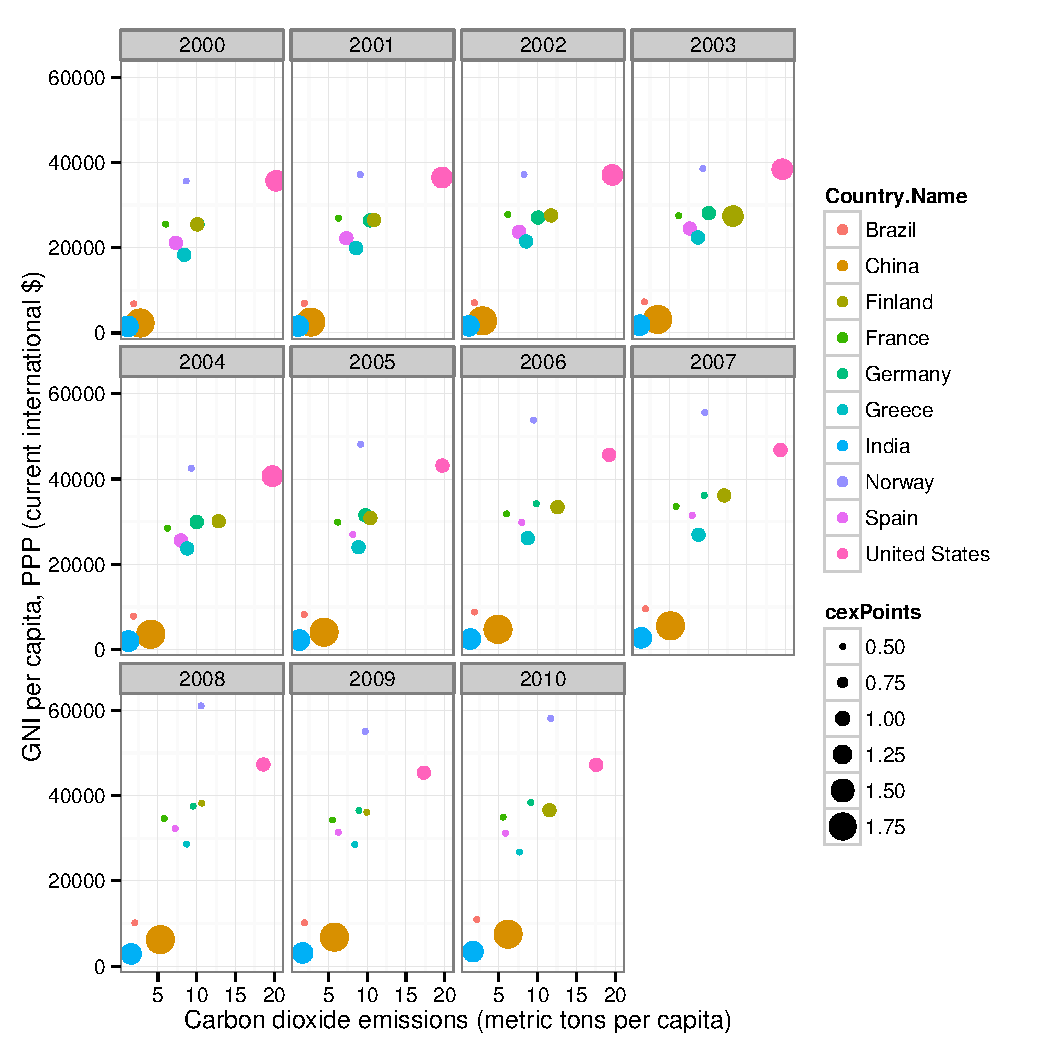
\includegraphics[width=.9\linewidth]{figs/CO2pointsGG.pdf}
\caption{\(\mathrm{CO_2}\) emissions versus GNI per capita for different intervals of the ratio of \(\mathrm{CO_2}\) emissions to the GDP PPP estimations. \label{fig:CO2pointsGG}}
\end{figure}

The \texttt{auto.key} mechanism of the \texttt{lattice} version is not able to cope with two grouping variables. Therefore, the legend, whose main componens are the labels (\texttt{intervals}) and the point sizes (\texttt{cex.key}), should be defined manually (Figure \ref{fig:CO2points}). 

\index{panel.text@\texttt{panel.text}}
\index{panel.groups@\texttt{panel.groups}}
\index{panel.superpose@\texttt{panel.superpose}}

\lstset{language=r,label= ,caption= ,captionpos=b,numbers=none}
\begin{lstlisting}
op <- options(digits = 2)
tab <- print(intervals)
options(op)
  
key <- list(space = 'right',
            title = expression(CO[2]/GNI.PPP),
            cex.title = 1,
            ## Labels of the key are the intervals strings
            text = list(labels = names(tab), cex = 0.85),
            ## Points sizes are defined with cex.key
            points = list(col = 'black', pch = 19,
                cex = cex.key, alpha = 0.7))

  
xyplot(GNI.capita ~ CO2.capita|factor(Year), data = CO2data,
       xlab = "Carbon dioxide emissions (metric tons per capita)",
       ylab = "GNI per capita, PPP (current international $)",
       groups = Country.Name, key = key, alpha = 0.7,
       panel  =  panel.superpose,
       panel.groups  =  function(x, y,
           subscripts, group.number, group.value, ...){
           panel.xyplot(x, y,
                        col  =  palOrdered[group.number],
                        cex  =  CO2data$cexPoints[subscripts])
           panel.pointLabel(x, y, labels = group.value,
                            col = palOrdered[group.number],
                            cex = 0.7)
       }
       ) 
\end{lstlisting}

\begin{figure}[htbp]
\centering
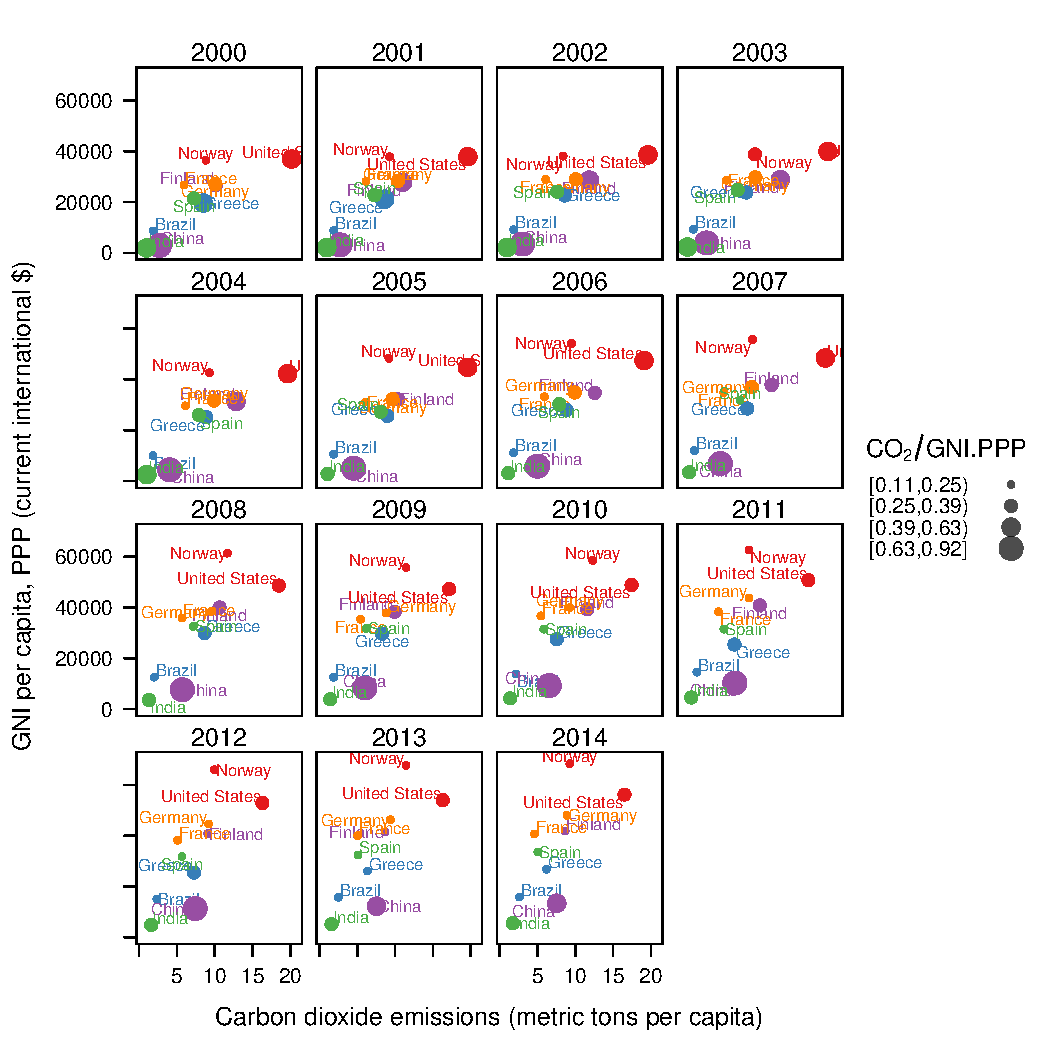
\includegraphics[width=.9\linewidth]{figs/CO2points.pdf}
\caption{\(\mathrm{CO_2}\) emissions versus GNI per capita for different intervals of the ratio of \(\mathrm{CO_2}\) emissions to the GDP PPP estimations. \label{fig:CO2points}}
\end{figure}

\section{Interactive}
\label{sec:orgefcc066}
\subsection{\texttt{googleVis}}
\label{sec:org472c658}
The first solution is a Motion Chart the \texttt{googleVis} package
\cite{Gesmann.deCastillo2011}, an interface between R and the Google
Visualisation API. With its \texttt{gvisMotionChart} function it is easy to
produce a Motion Chart that can be displayed using a browser with
Flash enabled (Figure \ref{fig:googleVis}).

\index{Packages!googleVis@\texttt{googleVis}}
\lstset{language=r,label= ,caption= ,captionpos=b,numbers=none}
\begin{lstlisting}
library(googleVis)
pgvis <- gvisMotionChart(CO2data,
                         idvar='Country.Name',
                         timevar='Year')
\end{lstlisting}

\begin{figure}
  \centering
  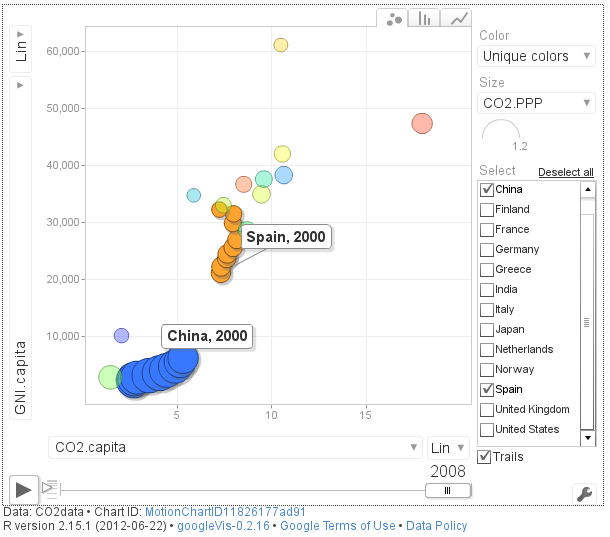
\includegraphics[width=\textwidth]{figs/googleVis}
  \caption{Snapshot of a Motion Chart produced with googleVis.}
  \label{fig:googleVis}
\end{figure}


Although the \texttt{gvisMotionChart} is quite easy to use, the global
appearance and behavior are completely determined by Google
API\footnote{You should read the Google API Terms of Service before using
\texttt{googleVis}: \url{https://developers.google.com/terms/}.}. Moreover, you should carefully read their Terms of Use
before using it for public distribution.


\subsection{plotly}
\label{sec:orga5a0d6e}

\index{Packages!plotlyG@\texttt{plotly}}

\lstset{language=r,label= ,caption= ,captionpos=b,numbers=none}
\begin{lstlisting}
library(plotly)

p <- plot_ly(CO2data,
             x = ~CO2.capita,
             y = ~GNI.capita,
             size = ~CO2.PPP, 
             text = ~Country.Name, hoverinfo = "text")

p <- add_markers(p,
                 color = ~Country.Name,
                 frame = ~Year,
                 ids = ~Country.Name,
                 showlegend = FALSE)

p <- animation_opts(p,
                    frame = 1000,
                    transition = 800,
                    redraw = FALSE) %>%
    animation_slider(
        currentvalue = list(prefix = "Year "))

p
\end{lstlisting}

\begin{figure}[htbp]
\centering
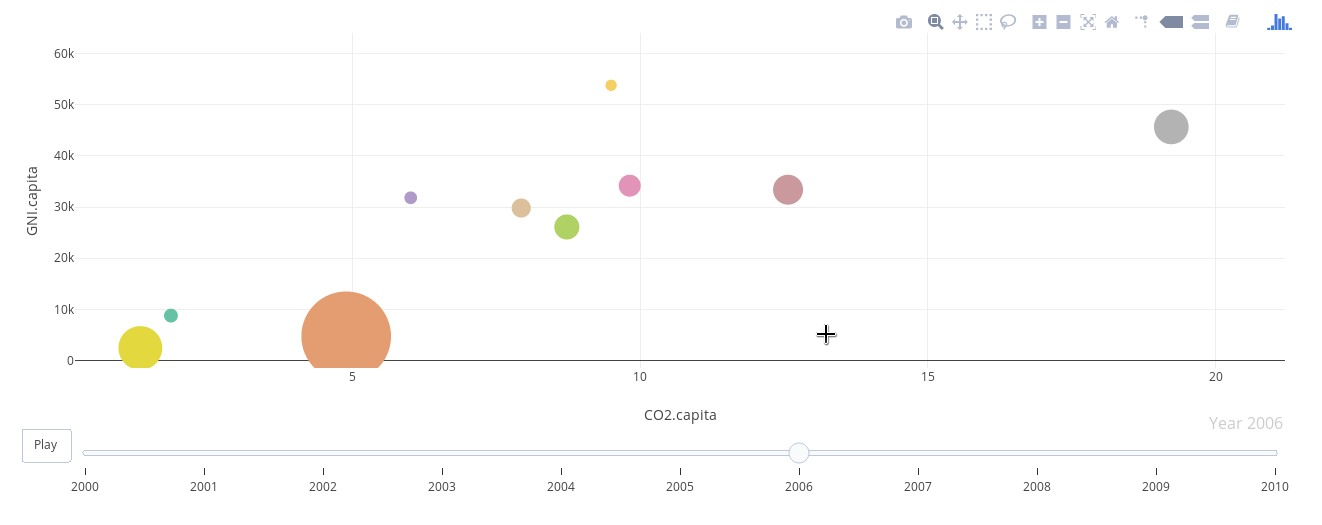
\includegraphics[width=.9\linewidth]{figs/plotly_animation.png}
\caption{plotly animation \label{fig:plotly_animation}}
\end{figure}

\subsection{\floweroneleft gridSVG}
\label{sec:org8efc594}
The final solution to display this multivariate time series is with
animation via the function \texttt{grid.animate} of the \texttt{gridSVG}
package. We will mimic the Trendalyzer/Motion Chart solution, using
traveling bubbles of different colors and with radius proportional to
\texttt{CO2.PPP}.

The first step is to draw the initial state of the bubbles. Their
colors are again defined by the \texttt{palOrdered} palette, although the
\texttt{adjustcolor} function is used for a ligther \texttt{fill} color. Because
there will not be a legend, there is no need to define class
intervals, and thus the radius is directly proportional to the value
of \texttt{CO2data\$CO2.PPP}.

\index{Packages!gridSVG@\texttt{gridSVG}}

\lstset{language=r,label= ,caption= ,captionpos=b,numbers=none}
\begin{lstlisting}
library(gridSVG)

xyplot(GNI.capita ~ CO2.capita,
       data = CO2data,
       xlab = "Carbon dioxide emissions (metric tons per capita)",
       ylab = "GNI per capita, PPP (current international $)",
       subset = Year==2000, groups = Country.Name,
       ## The limits of the graphic are defined
       ## with the entire dataset
       xlim = extendrange(CO2data$CO2.capita),
       ylim = extendrange(CO2data$GNI.capita),
       panel = function(x, y, ..., subscripts, groups) {
           color <- palOrdered[groups[subscripts]]
           radius <- CO2data$CO2.PPP[subscripts]
           ## Size of labels
           cex <- 1.1*sqrt(radius)
           ## Bubbles
           grid.circle(x, y, default.units = "native",
                       r = radius*unit(.25, "inch"),
                       name = trellis.grobname("points", type = "panel"),
                       gp = gpar(col = color,
                               ## Fill color ligther than border
                               fill = adjustcolor(color, alpha = .5),
                               lwd = 2))
           ## Country labels
           grid.text(label = groups[subscripts],
                     x = unit(x, 'native'),
                     ## Labels above each bubble
                     y = unit(y, 'native') + 1.5 * radius *unit(.25, 'inch'),
                     name = trellis.grobname('labels', type = 'panel'),
                     gp = gpar(col = color, cex = cex))
       })
\end{lstlisting}

From this initial state, \texttt{grid.animate} creates a collection of
animated graphical objects with the result of \texttt{animUnit}. This
function produces a set of values that will be interpreted by
\texttt{grid.animate} as intermediate states of a feature of the graphical
object. Thus, the bubbles will travel across the values defined by
\texttt{x\_points} and \texttt{y\_points}, while their labels will use \texttt{x\_points} and
\texttt{x\_labels}.

The use of \texttt{rep=TRUE} ensures that the animation will be repeated
indefinitely.

\index{animUnit@\texttt{animUnit}}
\index{grid.animate@\texttt{grid.animate}}

\lstset{language=r,label= ,caption= ,captionpos=b,numbers=none}
\begin{lstlisting}
## Duration in seconds of the animation
duration <- 20
  
nCountries <- nlevels(CO2data$Country.Name)
years <- unique(CO2data$Year)
nYears <- length(years)

## Intermediate positions of the bubbles
x_points <- animUnit(unit(CO2data$CO2.capita, 'native'),
                     id = rep(seq_len(nCountries), each = nYears))
y_points <- animUnit(unit(CO2data$GNI.capita, 'native'),
                     id = rep(seq_len(nCountries), each = nYears))
## Intermediate positions of the labels
y_labels <- animUnit(unit(CO2data$GNI.capita, 'native') +
                     1.5 * CO2data$CO2.PPP * unit(.25, 'inch'),
                     id = rep(seq_len(nCountries), each = nYears))
## Intermediate sizes of the bubbles
size <- animUnit(CO2data$CO2.PPP * unit(.25, 'inch'),
                 id = rep(seq_len(nCountries), each = nYears))

grid.animate(trellis.grobname("points", type = "panel", row = 1, col = 1),
             duration = duration,
             x = x_points,
             y = y_points,
             r = size,
             rep = TRUE)

grid.animate(trellis.grobname("labels", type = "panel", row = 1, col = 1),
             duration = duration,
             x = x_points,
             y = y_labels,
             rep = TRUE)

\end{lstlisting}

A bit of interactivity can be added with the \texttt{grid.hyperlink}
function. For example, the following code adds the corresponding
Wikipedia link to a mouse click on each bubble.

\index{grid.hyperlink@\texttt{grid.hyperlink}}

\lstset{language=r,label= ,caption= ,captionpos=b,numbers=none}
\begin{lstlisting}
countries <- unique(CO2data$Country.Name)
URL <- paste('http://en.wikipedia.org/wiki/', countries, sep = '')
grid.hyperlink(trellis.grobname('points', type = 'panel', row = 1, col = 1),
               URL, group = FALSE)
  
\end{lstlisting}

Finally, the time information: The year is printed in the lower
right corner, using the \texttt{visibility} attribute of an animated
\texttt{textGrob} object to show and hide the values.
\lstset{language=r,label= ,caption= ,captionpos=b,numbers=none}
\begin{lstlisting}
visibility <- matrix("hidden", nrow = nYears, ncol = nYears)
diag(visibility) <- "visible"
yearText <- animateGrob(garnishGrob(textGrob(years, .9, .15,
                                             name = "year",
                                             gp = gpar(cex = 2, col = "grey")),
                                    visibility = "hidden"),
                        duration = 20,
                        visibility = visibility,
                        rep = TRUE)
grid.draw(yearText)
\end{lstlisting}

The SVG file produced with \texttt{grid.export} is available at the website
of the book (Figure \ref{fig:bubblesSVG}). Because this animation does
not trace the paths, Figure \ref{fig:CO2-GNI-DL} provides this
information as a static complement.

\index{grid.export@\texttt{grid.export}}

\lstset{language=r,label= ,caption= ,captionpos=b,numbers=none}
\begin{lstlisting}
grid.export("figs/bubbles.svg")
\end{lstlisting}

\begin{figure}
  \centering
  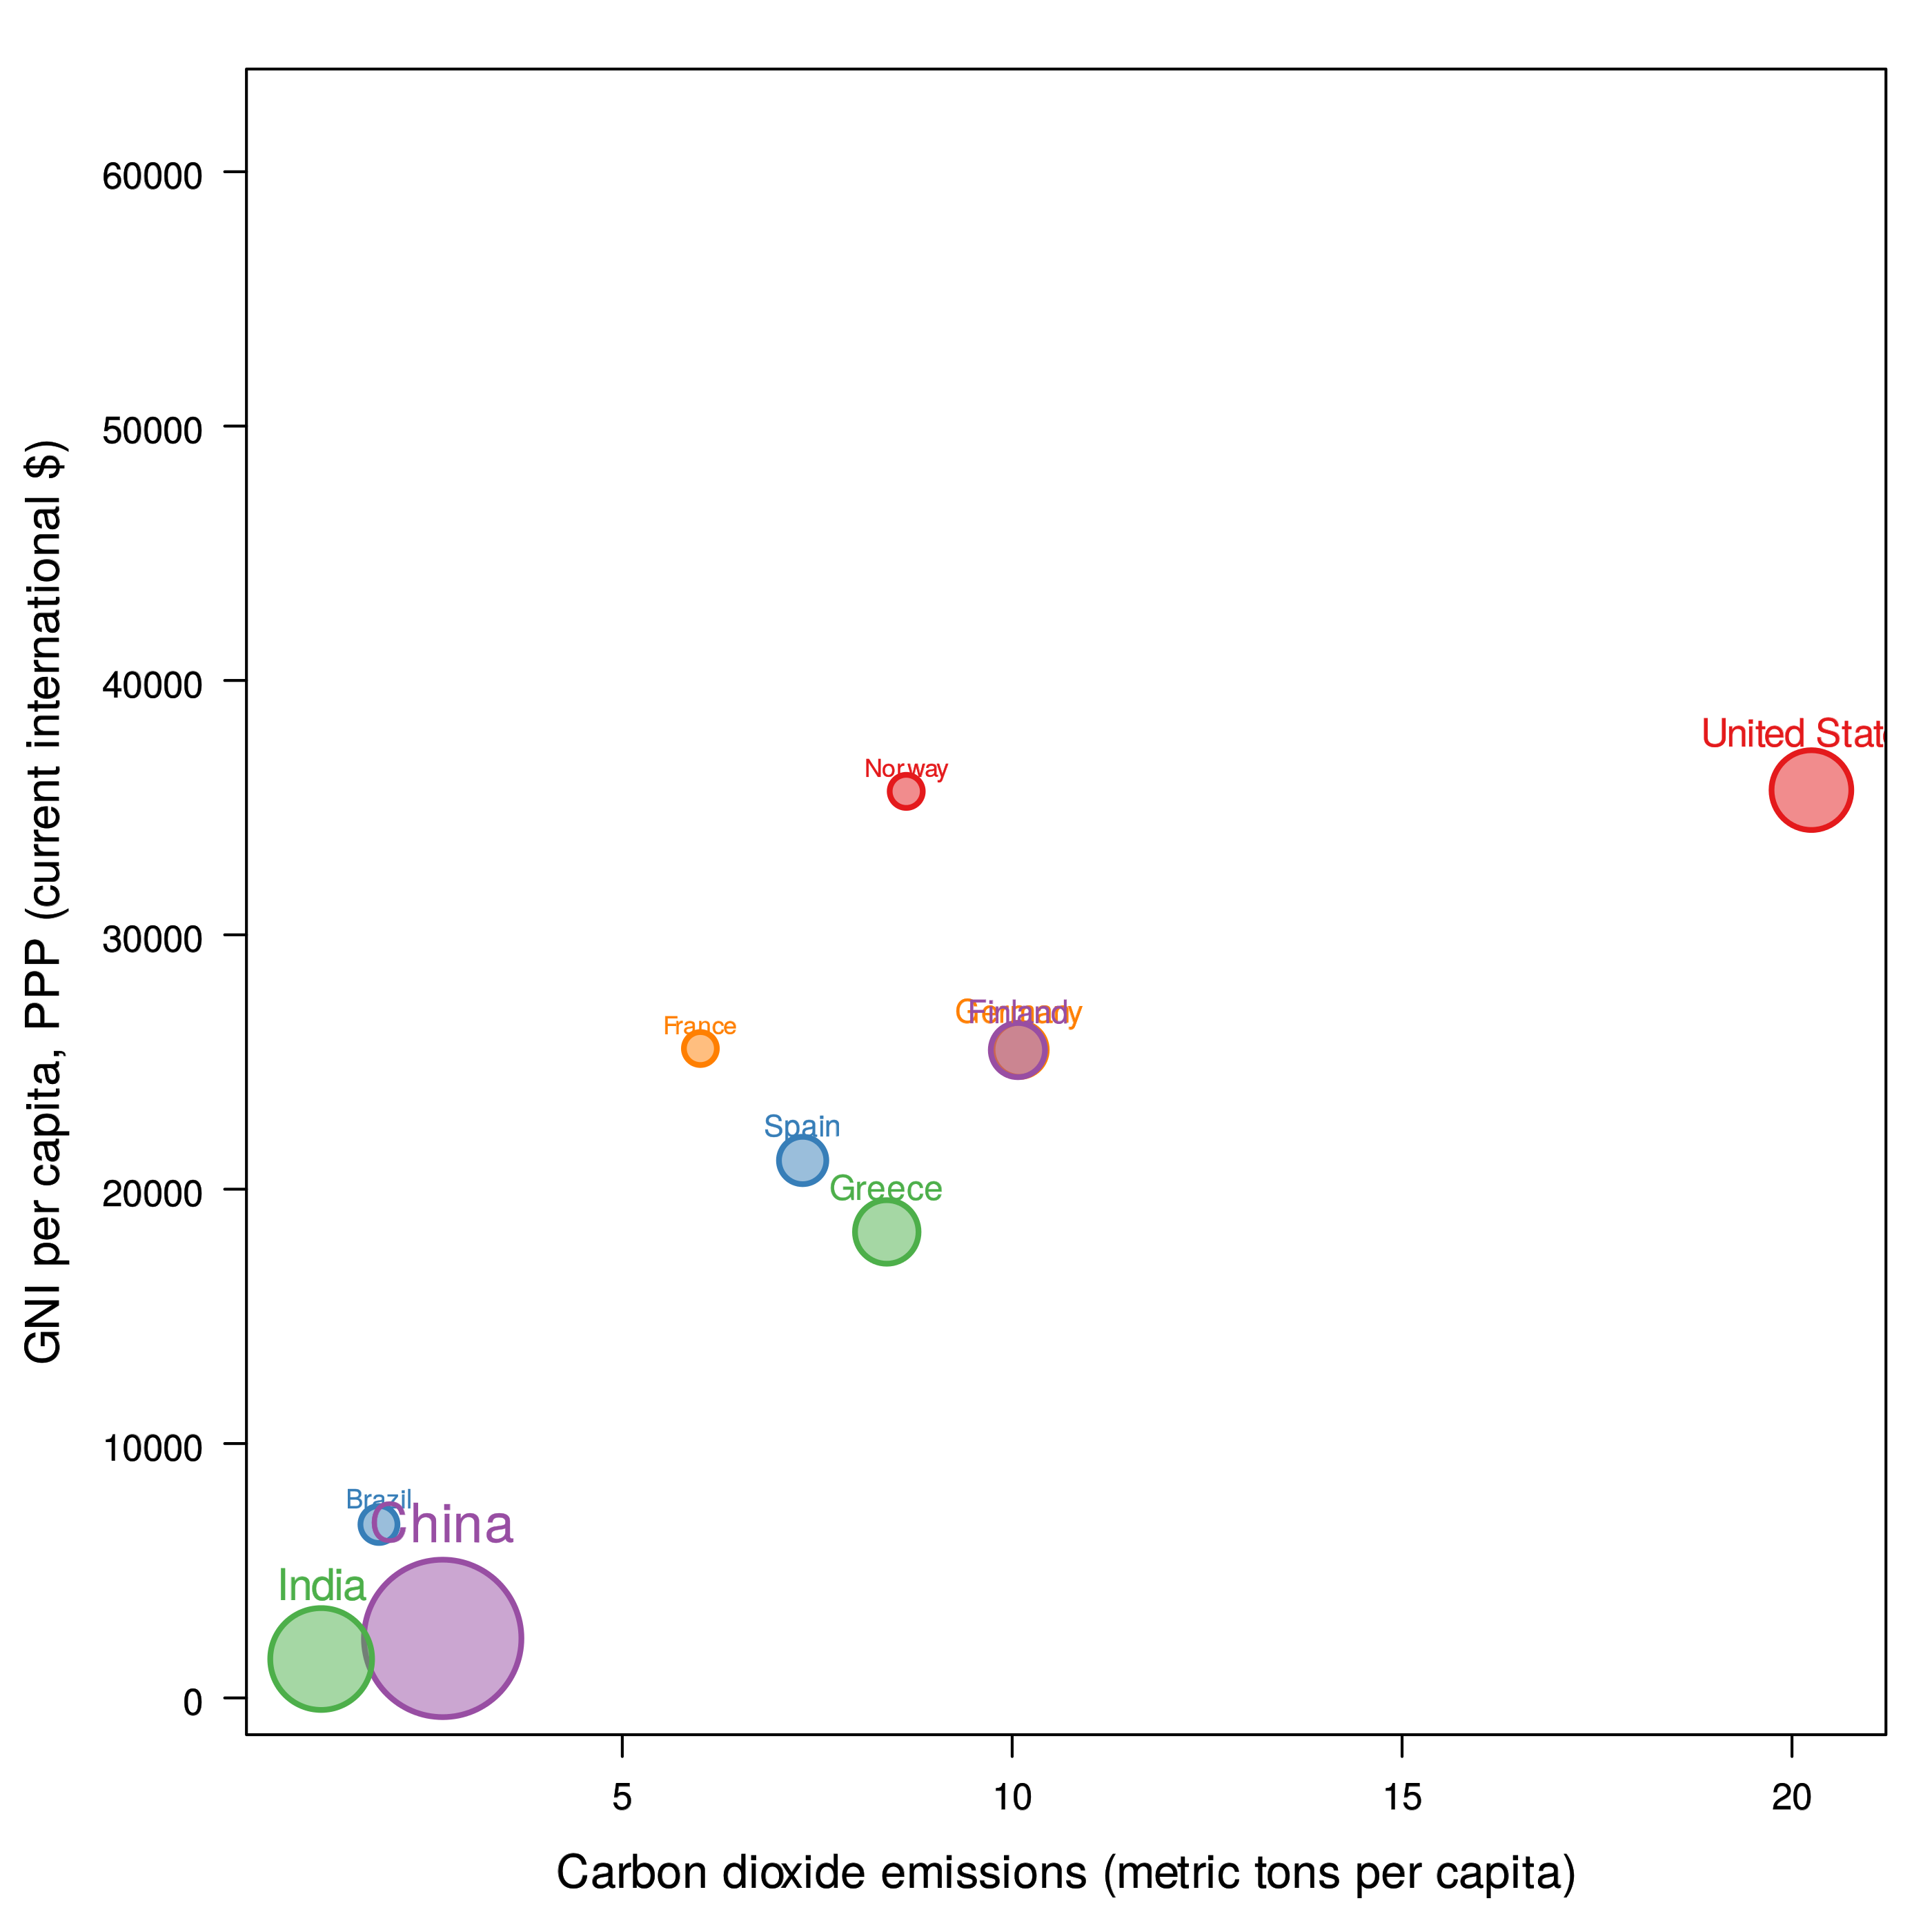
\includegraphics[width=\textwidth]{figs/bubbles.png}
  \caption{Animated bubbles produced with \texttt{gridSVG}.}
  \label{fig:bubblesSVG}
\end{figure}

Now, sit down in your favorite easy chair and watch the magistral
video ``200 Countries, 200 Years, 4 Minutes''\footnote{\url{http://www.gapminder.org/videos/200-years-that-changed-the-world-bbc/}}. After that, you are
ready to open the SVG file of traveling bubbles: It is easier, a short
time period with less than twenty countries.



\chapter{About the Data}
\label{cha:dataTime}


\section{SIAR}
\label{sec:org0ca2455}
\index{Data!SIAR}
\index{Data!Meteorological variables}

The Agroclimatic Information System for Irrigation (SIAR)
\cite{SIAR2011} is a free-download database operating since 1999,
covering the majority of the irrigated area of Spain.  This network
belongs to the Ministry of Agriculture, Food and Environment of Spain,
as a tool to predict and study meteorological variables for
agriculture. SIAR is composed of twelve regional centers and a
national center, aiming to centralize and depurate measurements from
the stations of the network. Figure \ref{fig:SIAR_map} displays the
stations over an altitude map. Some stations from the complete network
have been omitted, due to difficulties accessing their coordinates
or to incomplete or spurious data series\footnote{The name and location data of these stations are available at the \href{https://github.com/oscarperpinan/CMSAF-SIAR/blob/master/data/SIAR.csv}{GitHub repository} of the paper \cite{Antonanzas-Torres.Canizares.ea2013}.}.
\begin{figure}
  \centering
  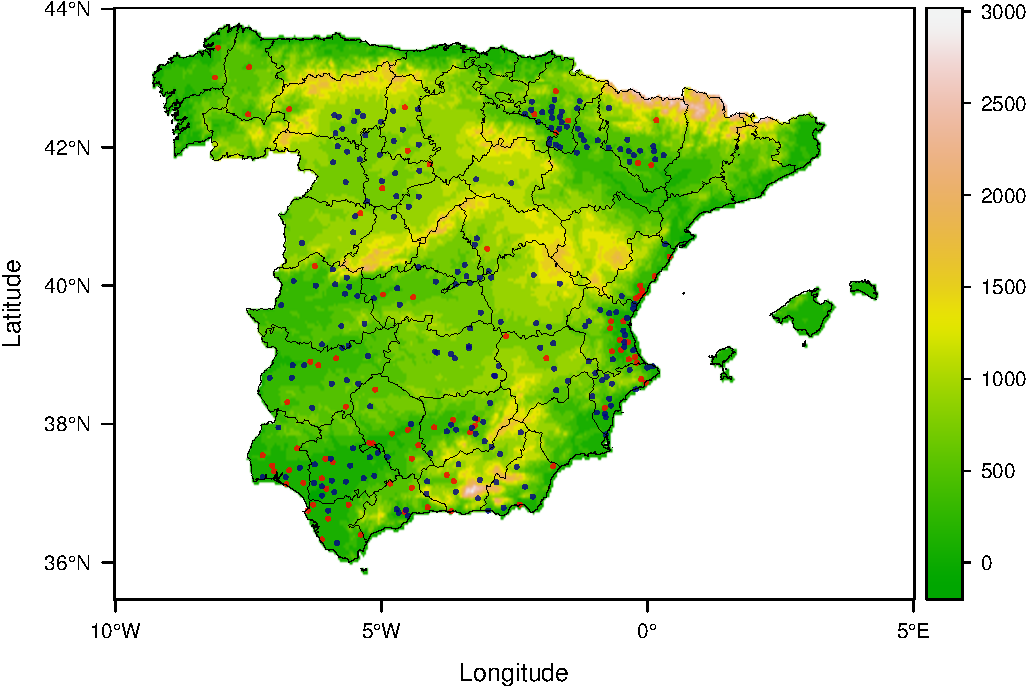
\includegraphics[width=\textwidth]{figs/mapaSIAR_crop}
  \caption{Meteorological stations of the SIAR network. The color key
    indicates the altitude (meters).}
  \label{fig:SIAR_map}
\end{figure}

\subsection{Daily Data of Different Meteorological Variables}
\label{sec:org1fd8a31}
As an example of multiple time series with different scales, we
will use 8 years (from January 2004 to December 2011) of daily
data corresponding to several meteorological variables measured at
the SIAR station located at Aranjuez (Madrid, Spain) available on
the SIAR webpage\footnote{\url{http://eportal.magrama.gob.es/websiar}}. The \texttt{aranjuez.gz} file, available in the
\texttt{data} folder of the book repository, contains this information
with several meteorological variables: average, maximum, and
minimum ambient temperature; average and maximum humidity; average
and maximum wind speed; rainfall; solar radiation on the
horizontal plane; and evotranspiration.

The \texttt{read.zoo} from the \texttt{zoo} package accepts this string and
downloads the data to construct a \texttt{zoo} object. Several
arguments are passed directly to \texttt{read.table} (\texttt{header}, \texttt{skip},
etc.) and are detailed conveniently on the help page of this
function. The \texttt{index.column} is the number of the column with the
time index, and \texttt{format} defines the date format of this index.

\index{Packages!zoo@\texttt{zoo}}
\index{read.zoo@\texttt{read.zoo}}

\lstset{language=r,label= ,caption= ,captionpos=b,numbers=none}
\begin{lstlisting}
  library(zoo)
  
  aranjuez <- read.zoo("data/aranjuez.gz",
                       index.column = 3, format = "%d/%m/%Y",
                       fileEncoding = 'UTF-16LE',
                       header = TRUE, fill = TRUE,
                       sep = ';', dec = ",", as.is = TRUE)
  aranjuez <- aranjuez[, -c(1:4)]
  
  names(aranjuez) <- c('TempAvg', 'TempMax', 'TempMin',
                       'HumidAvg', 'HumidMax',
                       'WindAvg', 'WindMax',
                       'Radiation', 'Rain', 'ET')
  
  
  summary(aranjuez)
\end{lstlisting}

\index{zoo@\texttt{zoo}}

From the summary it is clear that parts of these time series include erroneous outliers that can be
safely removed:
\lstset{language=r,label= ,caption= ,captionpos=b,numbers=none}
\begin{lstlisting}
  aranjuezClean <- within(as.data.frame(aranjuez),{
    TempMin[TempMin>40] <- NA
    HumidMax[HumidMax>100] <- NA
    WindAvg[WindAvg>10] <- NA
    WindMax[WindMax>10] <- NA
  })
  
  aranjuez <- zoo(aranjuezClean, index(aranjuez))
\end{lstlisting}


\subsection{Solar Radiation Measurements from Different Locations}
\label{sec:orgcf7f82f}
As an example of multiple time series with the same scale, we will use
data of daily solar radiation measurements from different locations.

\index{Data!Solar radiation}
\index{Data!SIAR}

Daily solar radiation incident on the horizontal plane is registered
by meterological stations and estimated from satellite images. This
meteorological variable is important for a wide variety of scientific
disciplines and engineering applications. Its variations and trends,
dependent on the location (mainly latitude, and also longitude and
altitude) and on time (day of the year), have been analyzed and
modeled in a huge collection of papers and reports. In this section
we will focus our attention on the time evolution of the solar
radiation. The spatial distribution and the spatio-time behavior will
be the subject of later sections.

The stations of the SIAR network include first-class pyranometers
according to the World Meteorological Organization (WMO), whose
absolute accuracy is within \(\pm 5\%\) and is typically lower than \(\pm
3\%\). Solar irradiance is recorded every 15 minutes and then
collated through a datalogger within the station to generate the daily
irradiation, which is later sent to the regional and national centers.

The file \texttt{navarra.RData} contains daily solar radiation data of 2011
from the meteorological stations of Navarra, Spain. The names of the
dataset are the abbreviations of each station name.


\section{Unemployment in the United States}
\label{sec:org33600b8}
As an example of time series that can be displayed both in individual
and in aggregate, we will use the unemployment data in the United
States. The information on unemployed persons by industry and class of
worker is available in Table A-14 published by the Bureau of Labor
Statistics\footnote{\url{http://www.bls.gov/webapps/legacy/cpsatab14.htm}}.

The dataset arranges the information with a row for each category
(\texttt{Series.ID}) and a column for each monthly value. In addition, there
are columns with the annual summaries (\texttt{annualCols}). We rearrange
this \texttt{data.frame}, dropping the \texttt{Series.ID} and the annual columns,
and transpose the data.

\index{Data!Unemployment}

\lstset{language=r,label= ,caption= ,captionpos=b,numbers=none}
\begin{lstlisting}
  unemployUSA <- read.csv('data/unemployUSA.csv')
  nms <- unemployUSA$Series.ID
  ##columns of annual summaries
  annualCols <- 14 + 13*(0:12)
  ## Transpose. Remove annual summaries
  unemployUSA <- as.data.frame(t(unemployUSA[,-c(1, annualCols)]))
  ## First 7 characters can be suppressed
  names(unemployUSA) <- substring(nms, 7)
  head(unemployUSA)
\end{lstlisting}

With the transpose, the column names of the original data set are
now the row names of the \texttt{data.frame}. The \texttt{as.yearmon} function
of the \texttt{zoo} package converts the character vector of names into a
\texttt{yearmon} vector, a class for representing monthly data. With
\texttt{Sys.setlocale("LC\_TIME", 'C')} we ensure that month abbreviations
(\texttt{\%b}) are correctly interpreted in a non-English locale. This
vector is the time index of a new \texttt{zoo} object. 

\index{Packages!zoo@\texttt{zoo}}
\index{as.yearmon@\texttt{as.yearmon}}
\index{apply@\texttt{apply}}
\index{zoo@\texttt{zoo}}

\lstset{language=r,label= ,caption= ,captionpos=b,numbers=none}
\begin{lstlisting}
  library(zoo)
  
  Sys.setlocale("LC_TIME", 'C')
  idx <- as.yearmon(row.names(unemployUSA), format='%b.%Y')
  unemployUSA <- zoo(unemployUSA, idx)
\end{lstlisting}

Finally, those rows with \texttt{NA} values are removed.
\lstset{language=r,label= ,caption= ,captionpos=b,numbers=none}
\begin{lstlisting}
  isNA <- apply(is.na(unemployUSA), 1, any)
  unemployUSA <- unemployUSA[!isNA,]
\end{lstlisting}

\section{Gross National Income and CO\(_{\text{2}}\) Emissions}
\label{sec:org6a96092}
The catalog data of the World Bank Open Data initiative includes a the
World Development Indicators (WDI)\footnote{\url{http://databank.worldbank.org/Data/Views/VariableSelection/SelectVariables.aspx}}. Among them we will analyze
the evolution of the relationship between Gross National Income (GNI)
and \(CO_2\) emissions for a set of countries. The package \texttt{WDI} is able
to search and download these data series.

\index{Data!World Bank} 
\index{Data!CO2@$CO_2$}
\index{Data!GNI}
\index{Packages!WDI@\texttt{WDI}}

\lstset{language=r,label= ,caption= ,captionpos=b,numbers=none}
\begin{lstlisting}
  library(WDI)
    
  CO2data <- WDI(indicator=c('EN.ATM.CO2E.PC', 'EN.ATM.CO2E.PP.GD',
                'NY.GNP.MKTP.PP.CD', 'NY.GNP.PCAP.PP.CD'),
            start=2000, end=2011,
            country=c('BR', 'CN', 'DE', 'ES',
                'FI', 'FR', 'GR', 'IN', 'NO', 'US'))

  names(CO2data) <- c('iso2c', 'Country.Name', 'Year',
                      'CO2.capita', 'CO2.PPP',
                      'GNI.PPP', 'GNI.capita')
\end{lstlisting}

Only two minor modifications are needed: Remove the missing values and
convert the \texttt{Country.Name} column into a \texttt{factor}. This first
modification will save problems when displaying the time series, and
the \texttt{factor} conversion will be useful for grouping.
\lstset{language=r,label= ,caption= ,captionpos=b,numbers=none}
\begin{lstlisting}
  isNA <- apply(is.na(CO2data), 1, any)
  CO2data <- CO2data[!isNA, ]

  CO2data$Country.Name <- factor(CO2data$Country.Name)
\end{lstlisting}



%%% Local Variables:
%%% TeX-master: "../main.tex"
%%% End: